El proyecto de investigación ARTEMIS es una iniciativa interdisciplinaria que reúne el trabajo de varios estudiantes de diferentes especialidades y campos. Este enfoque colaborativo permite abordar el proyecto desde diversas perspectivas, enriqueciendo así el desarrollo y la implementación de soluciones innovadoras. ARTEMIS se centra en el diseño y desarrollo de aplicaciones digitales interactivas. Estas han sido específicamente desarrolladas para realizar terapias de estimulación emocional a través del arte y la música, utilizando la tecnología como vehículo principal. Además, estas aplicaciones están diseñadas para ser intuitivas y accesibles, permitiendo a los usuarios interactuar con ellas de manera sencilla. Este proyecto tiene como objetivo integrar las últimas innovaciones tecnológicas con prácticas terapéuticas tradicionales, para potenciar los beneficios emocionales y psicológicos de los pacientes. A pesar de que cada uno de los estudiantes que conforman el equipo se ha centrado en líneas de investigación particulares, todos comparten objetivos comunes que han guiado sus esfuerzos hacia una meta colectiva.

Para contribuir al conocimiento científico y hacer funcionales las terapias diseñadas, las aplicaciones permiten la configuración por edades y patologías. Se definen pruebas psicométricas\footnote{Los test psicométricos son largos ya que consisten en alrededor de 30-40 preguntas. Al final de cada aplicación o sesión, se realizan preguntas rápidas del tipo termómetro.} al inicio y al final de la actividad, y los datos recogidos\footnote{La definición del perfil del paciente implica una entrevista entre el terapeuta y el paciente, donde se indaga acerca de su historia musical, gustos y características relacionadas con la música. El terapeuta será el encargado de introducir una serie de datos en la aplicación para optimizar esta fase.} de los pacientes se almacenan para su posterior consulta por el terapeuta. Los datos recogidos incluyen la edad, el nivel escolar, si se ha estudiado algún instrumento y el instrumento preferido del paciente. El perfil del paciente determina la complejidad musical en, por ejemplo, la composición interactiva. Un perfil con menos experiencia musical tendrá la capacidad de entender una complejidad musical menor o menos disonante, mientras que un perfil con más experiencia puede manejar una armonía más elaborada. Es importante mencionar que estas aplicaciones tienen una función de doble usuario en la que tanto el terapeuta como el paciente participan simultáneamente, cada uno con un rol específico. El terapeuta actúa como instructor, guiando al paciente en su interacción con la aplicación. 

La primera fase del proyecto ARTEMIS se ha enfocado en el tratamiento de la ansiedad infantil, utilizando la tecnología como vehículo para la transición emocional, complementándose con terapias tradicionales basadas en musicoterapia. La estructura de las sesiones terapéuticas es modular y se puede adaptar a las necesidades individuales del paciente. Cada sesión comienza con la definición del perfil del paciente y luego se selecciona una o más actividades vinculadas directamente a las líneas de investigación previamente definidas, en las que profundizaremos más en detalle en los próximos párrafos. Dentro de cada actividad, se han desarrollado una o más aplicaciones con distintos enfoques, que pueden ser utilizadas en función de las observaciones del terapeuta. Las actividades que han servido como punto de partida para el desarrollo de estas aplicaciones, y que han dado lugar a las líneas de investigación, son:

\begin{itemize}
	\item \textbf{Actividad 1 - Psicoeducación emocional:} esta primera actividad se enfoca en entender la emoción, específicamente la ansiedad, y en cómo combatirla. El educador, que en este caso es el terapeuta, proporciona de manera concisa información científica relevante para responder a preguntas importantes. El paciente recibe una serie de herramientas que le ayudan a identificar, comprender y manejar la ansiedad.
	\item \textbf{Actividad 2 - Relajación guiada mediante la respiración:} el terapeuta, con la ayuda del soporte digital, guía al paciente a realizar ejercicios de relajación centrados en la respiración. El paciente sincroniza sus respiraciones con la interacción tecnológica, aportando un elemento artístico que acompaña la respiración.
	\item \textbf{Actividad 3 - Ordenar pensamientos a través del ritmo:} el paciente se centra en utilizar el ritmo como herramienta para organizar sus pensamientos y emociones. Bajo la guía del terapeuta, se establece un escenario rítmico que permite al paciente explorar y organizar sus ideas y sentimientos de una manera ordenada, respetando siempre su subjetividad.
	\item \textbf{Actividad 4 - Improvisación:} se basa en la completa libertad del paciente, donde, a través de la improvisación musical, el paciente debe expresar su estado de ánimo.
	\item \textbf{Actividad 5 - Repetición de patrones rítmicos:} el paciente debe escuchar y repetir patrones rítmicos con la mayor precisión posible con el objetivo de controlar la impulsividad. 
\end{itemize}

Estas actividades constituyen la base sobre la que se han construido para las distintas aplicaciones, respaldadas por las líneas de investigación. Estas líneas se han establecido para abordar los objetivos del proyecto desde una perspectiva multidisciplinaria, uniendo las cuatro áreas de estudio: arte, tecnología, música y terapias de estimulación emocional. Las líneas de investigación son las siguientes:

\begin{itemize}
	\item Musicoterapia y narrativa audiovisual.
	\item Musicoterapia y arte digital.
	\item Musicoterapia y composición interactiva.
	\item Musicoterapia y diseño de videojuegos (serious games).
	\item UX/UI interacción y branding.
\end{itemize}

Abordaremos cada línea de investigación individualmente, indagando en profundidad en sus aplicaciones derivadas. Específicamente, la aplicación más relevante para este TFG se encuentra en la línea de investigación de diseño de videojuegos con musicoterapia. Dejaremos esta para el final con el fin de explicarla en mayor detalle, ya que es él núcleo principal de este trabajo.

\section{Musicoterapia y narrativa audiovisual}

La narrativa audiovisual es una parte integral del proyecto de investigación. Está presente en todas las aplicaciones, en mayor o menor medida, y actúa como un vínculo entre todas ellas. El objetivo de contar una historia es proporcionar información al paciente de manera que pueda sentirse identificado y conectar directamente con sus emociones. Dado que estamos estudiando la ansiedad, es importante explicar al paciente cómo funciona e involucrarlo en la explicación integrada en forma de historia. Hemos definido tres elementos en la narrativa que están directamente relacionados con este enfoque, y cuyo objetivo es involucrar activamente al paciente.

\begin{itemize}
	\item \textbf{Personaje principal:} es el elemento más crítico de la narrativa. Su función es actuar como un espejo que permite al paciente identificarse, y sirve como guía para el mismo. Este personaje es una especie de Pepito Grillo\footnote{Pepito Grillo es un personaje de ficción creado para Las Aventuras de Pinocho (\cite{LADP:1883}), que Walt Disney Pictures, actual Walt Disney Studios, adaptó en 1940 en la película de animación Pinocho. En la cultura popular, Pepito Grillo representa una figura de confianza a quien recurrimos para obtener consejo. Esta figura nos ayuda a identificar nuestros errores y no teme cuestionarnos cuando nos equivocamos.}, cuyo objetivo es ayudar al paciente a comprender su problema y a encontrar una solución.
	\item \textbf{Nivel de explicación:} dependiendo de la edad a la que se dirige la narrativa, el nivel de profundidad debe variar y adaptarse\footnote{Por ejemplo, los niños pequeños suelen utilizar el pensamiento mágico, como un duende malo que nos pone nerviosos, mientras que los adolescentes necesitan ejemplos más concretos y realistas.}. El objetivo es lograr que el paciente se identifique con el ejemplo situacional que la historia propone. Para que esto suceda, es esencial usar analogías para explicar las leyes del mundo.
	\item \textbf{Píldoras mínimas:} para que la historia sirva como un nexo cohesivo entre las aplicaciones, debe quedar claro cuál es el objetivo de la actividad específica que se va a realizar. Debe responder a la pregunta: ¿Cuál es la finalidad de lo que estoy a punto de hacer?
\end{itemize}

Todos estos elementos se centran en lo que se conoce como inmersión contextual. Esto implica el estudio del contexto de los pacientes para introducir elementos que se ajusten a las circunstancias de cada uno. El objetivo es promover una identificación adecuada entre el paciente, su situación y la historia.

La historia principal debe unir todas las actividades de forma natural sin perder el objetivo que acabamos de comentar. Esta historia, escrita por Isabel Xiaowei de San Sebastián para ARTEMIS, se puede resumir de la siguiente manera:

\begin{adjustwidth}{100pt}{0pt}
	\noindent "\textit{El protagonista es un ser del bosque que nació de una flor, gracias al poder de una ninfa. La diosa Artemis ha perdido su magia y el protagonista ayuda a recuperarla. Su misión es buscar semillas de diente de león perdidas en el bosque para entregárselas a la ninfa, quien las transforma en flores. En su travesía, se encuentra con varios desafíos, representados por actividades terapéuticas, que debe completar para avanzar. El nivel no concluye hasta que se completan todas las actividades. Una vez finalizado un nivel, el protagonista puede repetirlo o continuar con la historia. Las ninfas, en intervalos regulares, se reúnen con las distintas flores de cada emoción que han creado a partir de las semillas y se las entregan a Artemis. Cada emoción se representa como una planta distinta, personalizando así la estética del personaje con diferentes plantas. Existe una escala del dolor que, dependiendo del nivel de ansiedad del paciente, muestra diferentes elementos que ayuden al terapeuta a comprender la situación del paciente.}"
\end{adjustwidth}

La ambientación de esta historia está fuertemente vinculada con la naturaleza, que se asocia con la relajación y vitalidad. Así, los elementos estéticos deben ser coherentes con este tema. Considerando que ARTEMIS se centra en la ansiedad infantil, los elementos estéticos se diseñan para adecuarse a este contexto. Esta estética, repleta de colores vivos y personajes con rasgos de la animación tradicional, busca establecer una conexión con su público objetivo. Como no podemos determinar el género del paciente que utilizará la aplicación, decidimos desde el principio que el personaje debía ser andrógino. En la \autoref{fig:MainCharacterConcept}, observamos que se intentó alcanzar este objetivo desde las primeras propuestas estéticas. La versión final del personaje mantiene la androginia, combinando rasgos humanos con elementos naturales. Se puede comparar la versión inicial con la final en la \autoref{fig:MainCharacter}.

\begin{figure}[h!]
	\centering
	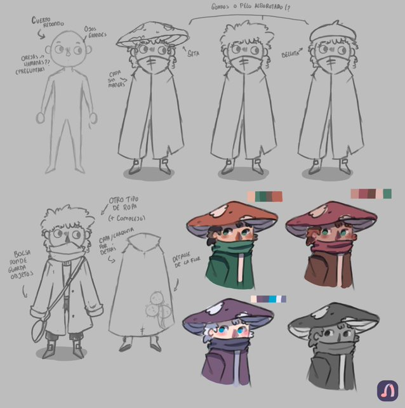
\includegraphics[width=0.4\linewidth]{Figuras/Desarrollo/PersonajesNuevosConcept}
	\caption{Propuesta inicial de personaje principal.}
	\label{fig:MainCharacterConcept}
	\vspace{-20pt}
\end{figure}

\begin{center}
	\textbf{Fuente:} Realizado por Sergio Calvo, miembro ARTEMIS.
\end{center}

\begin{figure}[h!]
	\centering
	\subfigure[Primera iteración del personaje.]{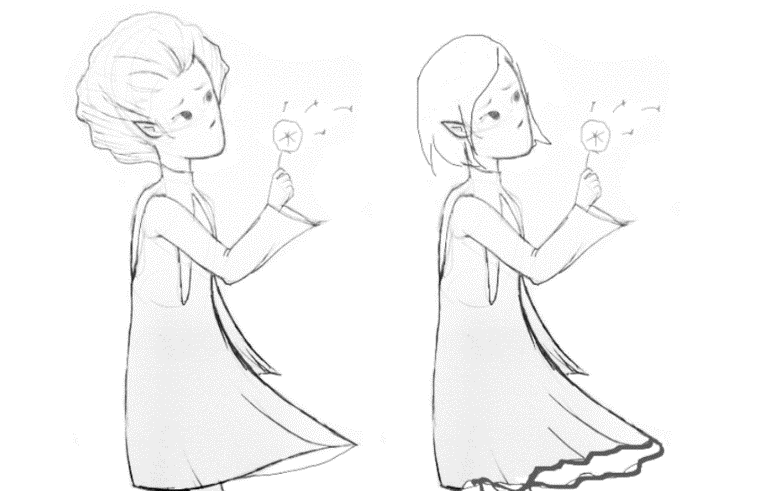
\includegraphics[width=0.4\textwidth]{./Figuras/Desarrollo/PersonajesAntiguos.png}\label{fig:MainCharacterOld}}
	\hfil
	\subfigure[Última iteración del personaje.]{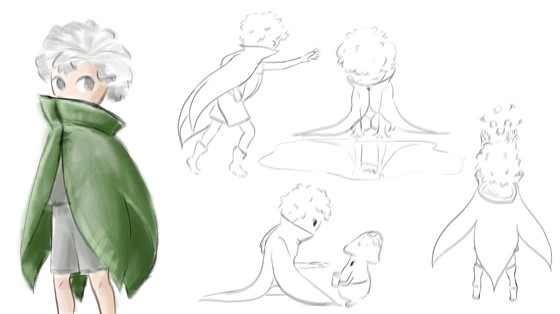
\includegraphics[width=0.4\textwidth]{./Figuras/Desarrollo/PersonajesNuevos.jpg}\label{fig:MainCharacterNew}}
	\caption{Evolución de la conceptualización del personaje principal.}
	\label{fig:MainCharacter}
	\vspace{-25pt}
\end{figure}

\begin{center}
	\textbf{Fuente:} Realizado por Isabel Xiaowei de San Sebastián, miembro ARTEMIS.
\end{center}

Las ninfas, musas y gracias tienen una fuerte relación con la música y pueden ser los personajes identificados con instrumentos que el protagonista encuentra en su aventura. Por esta razón, los personajes secundarios que el protagonista encuentra a lo largo de la narrativa portan instrumentos (como se puede observar en la \ref{fig:InstrumentCharacters}), representando físicamente a estos seres.

\begin{figure}[h!]
	\centering
	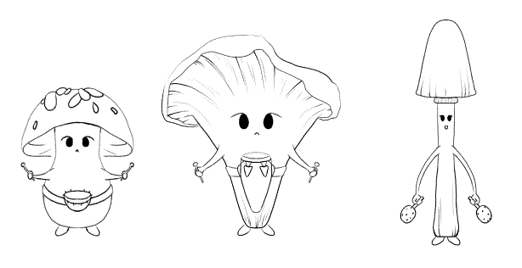
\includegraphics[width=0.3\linewidth]{Figuras/Desarrollo/InstrumentCharacters}
	\caption{Propuesta de concepto de personajes con instrumentos.}
	\label{fig:InstrumentCharacters}
	\vspace{-30pt}
\end{figure}

\begin{center}
	\textbf{Fuente:} Realizado por Isabel Xiaowei de San Sebastián, miembro ARTEMIS.	
\end{center}

Antes de concluir esta línea de investigación, es relevante describir el formato que fundamenta esta historia y cómo se lleva a cabo la interacción del paciente bajo la guía del terapeuta. La historia se visualiza a través de un libro ilustrado interactivo. De este modo, el terapeuta puede controlar el ritmo de la historia y, si es necesario, retroceder. Para avanzar, se debe pulsar manualmente el botón de pasar página, permitiendo al terapeuta determinar cuánto tiempo se necesita en cada página, en caso de tener que explicar algún detalle.
La ansiedad tiende a inquietar a quien la padece. Por ello, un sistema que permite adaptar el ritmo de la narrativa a cada situación, permite al terapeuta elegir el enfoque más beneficioso para el paciente en cuestión.

\begin{figure}[h!]
	\centering
	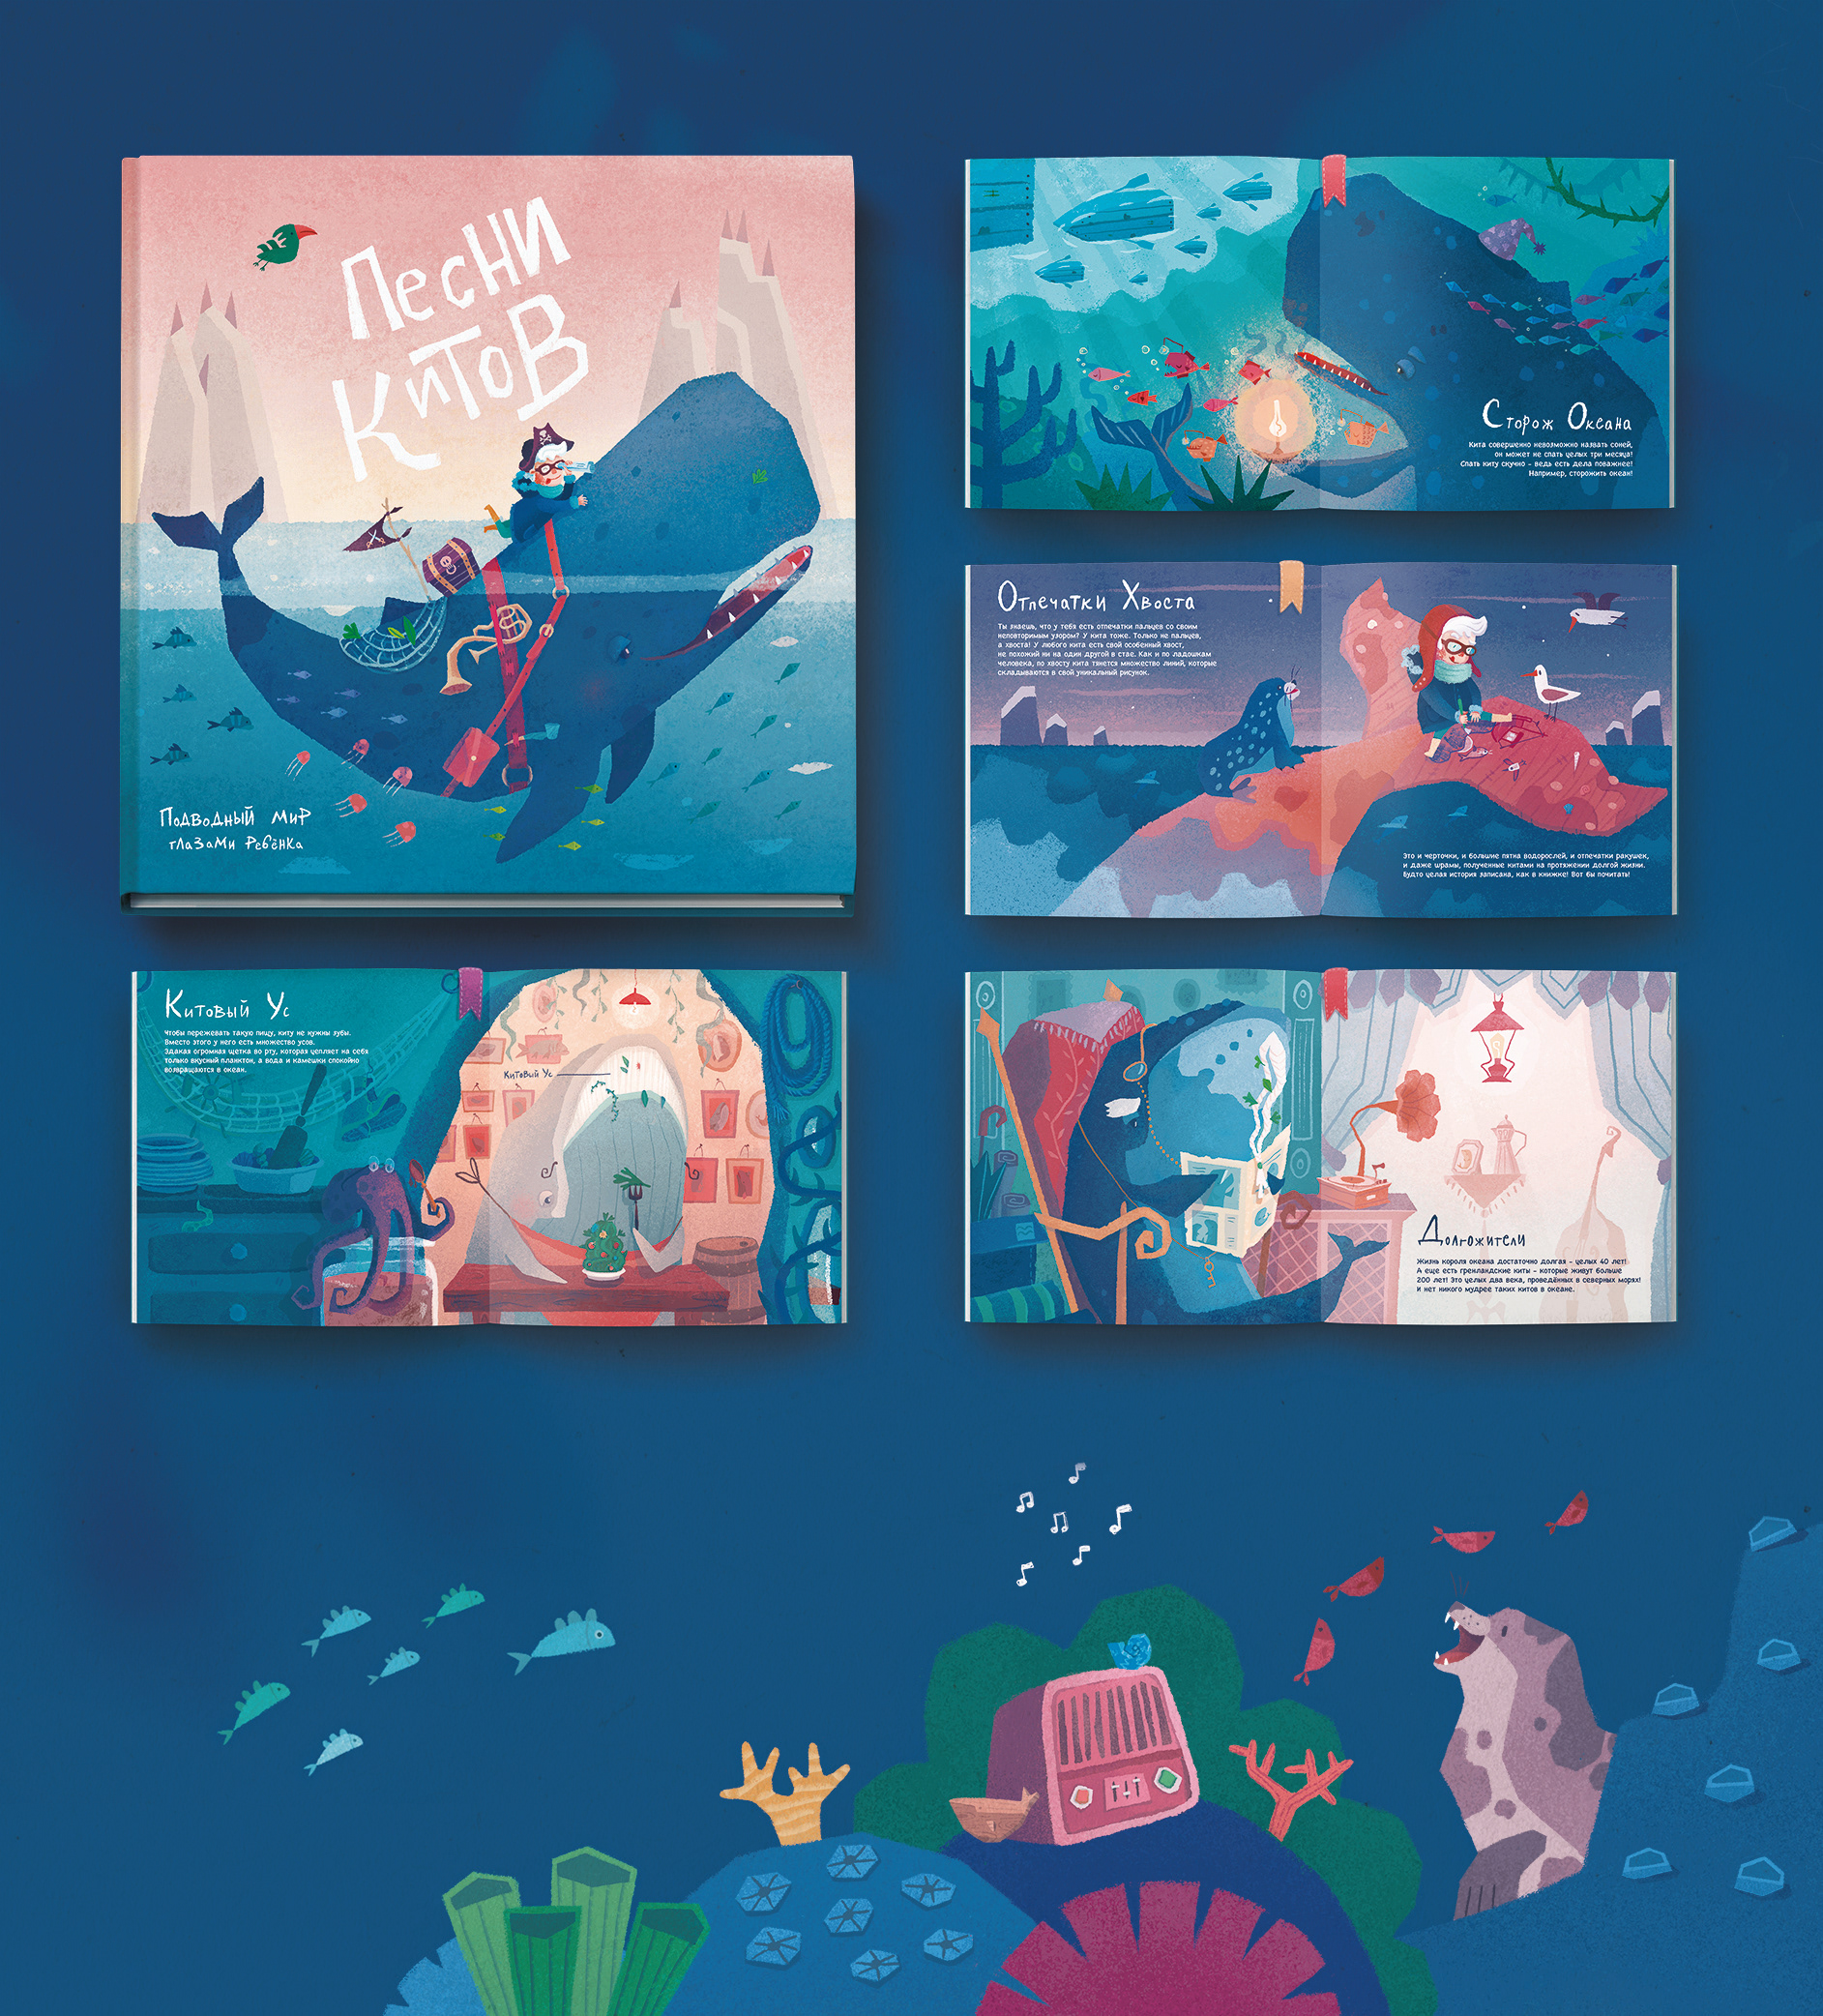
\includegraphics[width=0.4\linewidth]{Figuras/Desarrollo/ImagenReferenciaLibro.jpg}
	\caption{Imagen de referencia de libro interactivo.}
	\label{fig:LoriRiBook}
	\vspace{-30pt}
\end{figure}

\begin{center}
	\textbf{Fuente:} \citeauthor{LORIRI:2018} (\citeyear{LORIRI:2018}).	
\end{center}

\begin{figure}[h!]
	\centering
	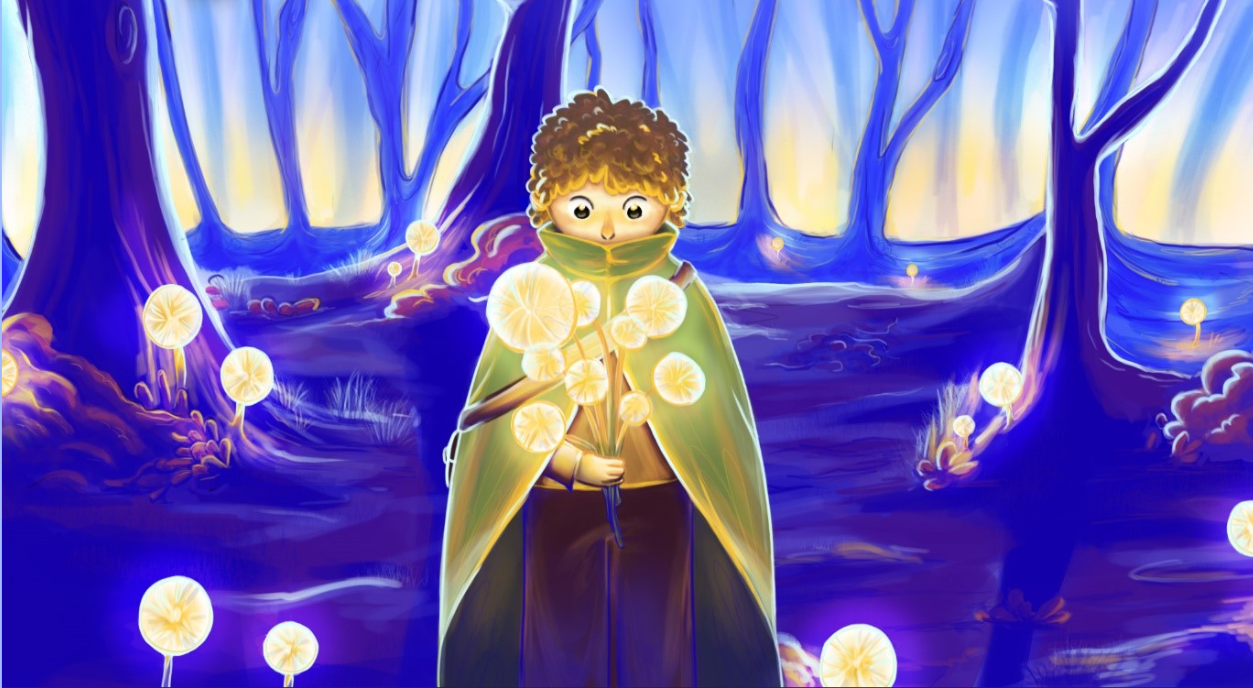
\includegraphics[width=0.5\linewidth]{Figuras/Desarrollo/IlustracionLibro.png}
	\caption{Ilustración de ejemplo del libro ilustrado interactivo.}
	\label{fig:BookIllustration}
	\vspace{-30pt}
\end{figure}

\begin{center}
	\textbf{Fuente:} Realizado por Isabel Xiaowei de San Sebastián, miembro ARTEMIS.
\end{center}

La narrativa es un elemento fundamental para la identificación del paciente con la aplicación. Esta aumenta la eficacia de la terapia en función del grado de inmersión que la tecnología pueda proporcionar en las sesiones de musicoterapia.

\section{Musicoterapia y arte digital}

La línea de investigación en arte digital propone una pieza de arte digital interactiva. Esta pieza, mediante experiencias visuales y música, puede ayudar en la gestión emocional y facilitar la transición de una emoción a otra a través de la interacción del usuario. Los datos de interacción se pueden recoger a través de la información proporcionada por periféricos comunes como una tableta y sus sensores (cámara o pantalla táctil). El objetivo de este recurso es ayudar al paciente a concentrarse y relajarse, enseñándole cómo respirar visualmente en situaciones de ansiedad. La interacción con esta herramienta se realiza mediante pulsaciones táctiles, ya sean cortas o prolongadas, o movimientos de la mano frente a la cámara. Se espera que estas acciones sean guiadas por el terapeuta para alcanzar su objetivo. De esta manera, al no usar un micrófono que puede generar varios problemas dependiendo del tipo de paciente que recibe la terapia\footnote{Usar un micrófono como sistema principal de entrada puede causar problemas en ciertos casos aislados. Las voces más graves producen ondas de sonido que son más difíciles de capturar, por lo que no sería correcto limitar las terapias a personas con voces más reconocibles.}, se evitan complicaciones. En términos de salida de la experiencia, la parte visual se mostrará en la pantalla y la parte musical se emitirá a través de altavoces o auriculares. Las propuestas de visualización para esta pieza se pueden dividir en dos categorías: visual y musical.

\begin{itemize}
	\item \textbf{Apartado visual:} se genera un mar de partículas que oculta un paisaje, siguiendo la línea estética del proyecto. Este paisaje se revela mediante la animación de las partículas, las cuales se ven afectadas por el contacto del dedo del paciente al deslizarse por la pantalla. Este movimiento depende de la longitud de la exhalación.
	\item \textbf{Apartado musical:} se reproduce una melodía relajante de fondo con sonidos que nos recuerdan a la naturaleza (el viento, la vegetación, los animales, etc). Por otro lado, al interactuar con la pieza, también se emite un sonido más fuerte de brisa, que emula la exhalación.
\end{itemize}



\begin{figure}[h!]
	\centering
	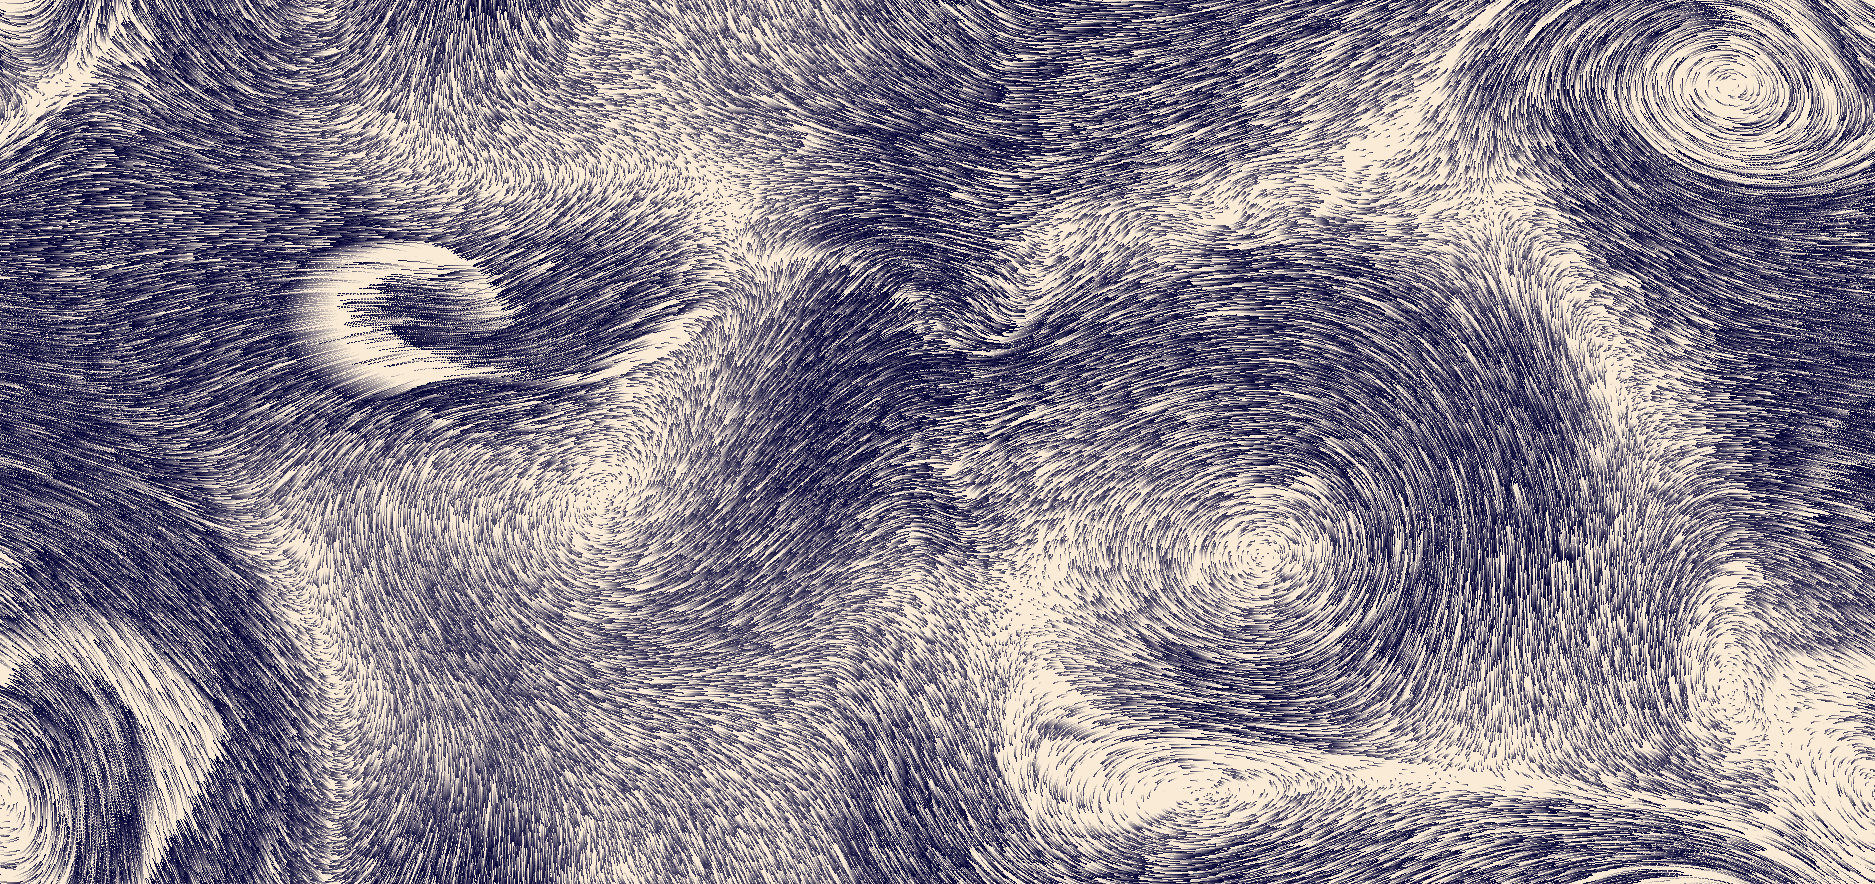
\includegraphics[width=0.4\linewidth]{Figuras/Desarrollo/MarParticulas.png}
	\caption[Referencia principal de arte interactivo Vamoss.]{Referencia principal de arte interactivo en relación con la propuesta de Clara Guoshi, miembro de ARTEMIS. En el enlace de la referencia bibliográfica, se puede probar la experiencia creada por Vamoss.}
	\label{fig:SeaParticles}
	\vspace{-40pt}
\end{figure}

\begin{center}
	\textbf{Fuente:} \citeauthor{VAMOSS:2023} (\citeyear{VAMOSS:2023}).
\end{center}

\section{Musicoterapia y composición interactiva}

La composición interactiva se basa en la creación de música como una forma de expresión libre. Mediante la modificación en tiempo real de un tema musical o combinaciones musicales, se pueden generar variaciones melódicas y paisajes sonoros. A través de esta interacción, el paciente puede crear música sencilla. Esta línea de investigación presenta dos aplicaciones. Aunque son diferentes, ambas buscan utilizar los mismos métodos para alcanzar el objetivo.

\subsection{Aplicación 1: Paisaje sonoro}

El paisaje sonoro, que se inspira en referencias como \textit{Reactable}\footnote{Reactable es un instrumento musical electrónico colaborativo desarrollado por el Grupo de Tecnología Musical de la Universidad Pompeu Fabra en Barcelona. Este instrumento permite a los usuarios crear topologías musicales complejas y dinámicas mediante la colocación y rotación de elementos físicos en su interfaz. Está inspirado en los sintetizadores modulares de los años sesenta y permite el uso de generadores, filtros y moduladores para la creación musical.} o \textit{Incredibox} (\citeauthor{INCREDIBOX:2023}, \citeyear{INCREDIBOX:2023}), se centra en la creación de música a través de la selección de los instrumentos que participarán en la melodía. Esta aplicación tiene como objetivo acomodar a aquellos pacientes con menor conocimiento musical, reforzando la simplicidad requerida para que estas aplicaciones sean utilizadas por su público objetivo. En realidad, no existe una solución incorrecta, lo que permite al paciente sentir que tiene el control de la música y evitar la frustración de no poder crear una melodía armoniosa.

La aplicación consta de cuatro niveles distintos, cada uno asociado a un género musical. Esto permite al terapeuta seleccionar los instrumentos con los que desea trabajar, en función de las necesidades del paciente. Además, la aplicación puede utilizarse de manera indefinida, hasta que el paciente o el terapeuta decidan finalizar su uso. La idea principal de la aplicación es que los instrumentos generan un paisaje musical, asociando cada elemento con aspectos de la naturaleza, como flores o árboles. Este paisaje cambia según el género musical seleccionado. Los cuatro géneros que agrupan los distintos instrumentos, junto con algunos ejemplos de instrumentos, son:

\begin{itemize}
	\item \textbf{Música clásica:} piano, violín, viola, trompeta, trombón, percusión, violonchelo, oboe, corno, fagot, clarinete, contrabajo, flauta traversa o flauta de pico.
	\item \textbf{Música pop-rock:} voz, guitarra eléctrica, bajo, batería, teclados, guitarra acústica, sintetizador o caja de ritmos.
	\item \textbf{Música caribeña o latina:} gaitas, arco musical, caña de millo, guacharaca, guache, tablitas, bombos, redoblantes, platillos, campanas o tambor.
	\item \textbf{Música electrónica:} sintetizador, caja de ritmos, theremin o sonidos generados por ordenador.
\end{itemize}

Cada uno de estos géneros representa un paisaje específico, aludiendo a las cuatro estaciones. Los elementos de fondo y la paleta de colores cambian, pero siempre se mantiene el aspecto natural.La aplicación, desarrollada por Ángela García, miembro de ARTEMIS, incluye un menú inicial donde se puede seleccionar el género deseado y la pantalla de juego, donde se puede observar en acción lo que hemos mencionado anteriormente. En la \autoref{fig:SonoricEnvironment}, se pueden observar ambas interfaces.

\begin{figure}[h!]
	\centering
	\subfigure{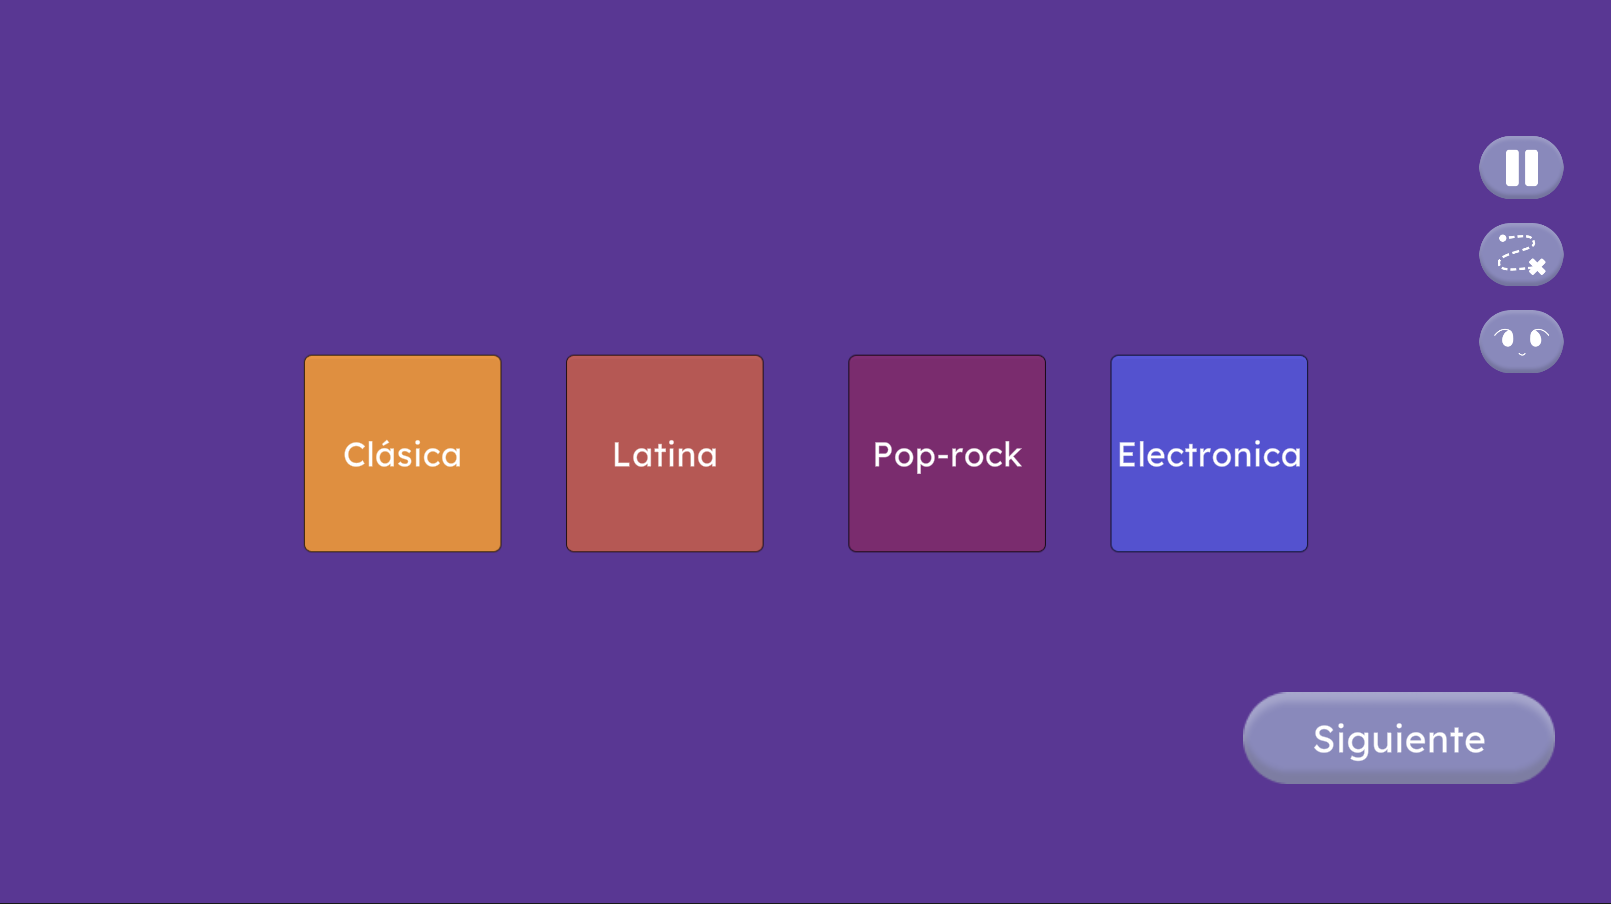
\includegraphics[width=0.4\textwidth]{./Figuras/Desarrollo/PaisajeSonoroMenu.png}\label{fig:SonoricEnvironmentMenu}}
	\hfil
	\subfigure{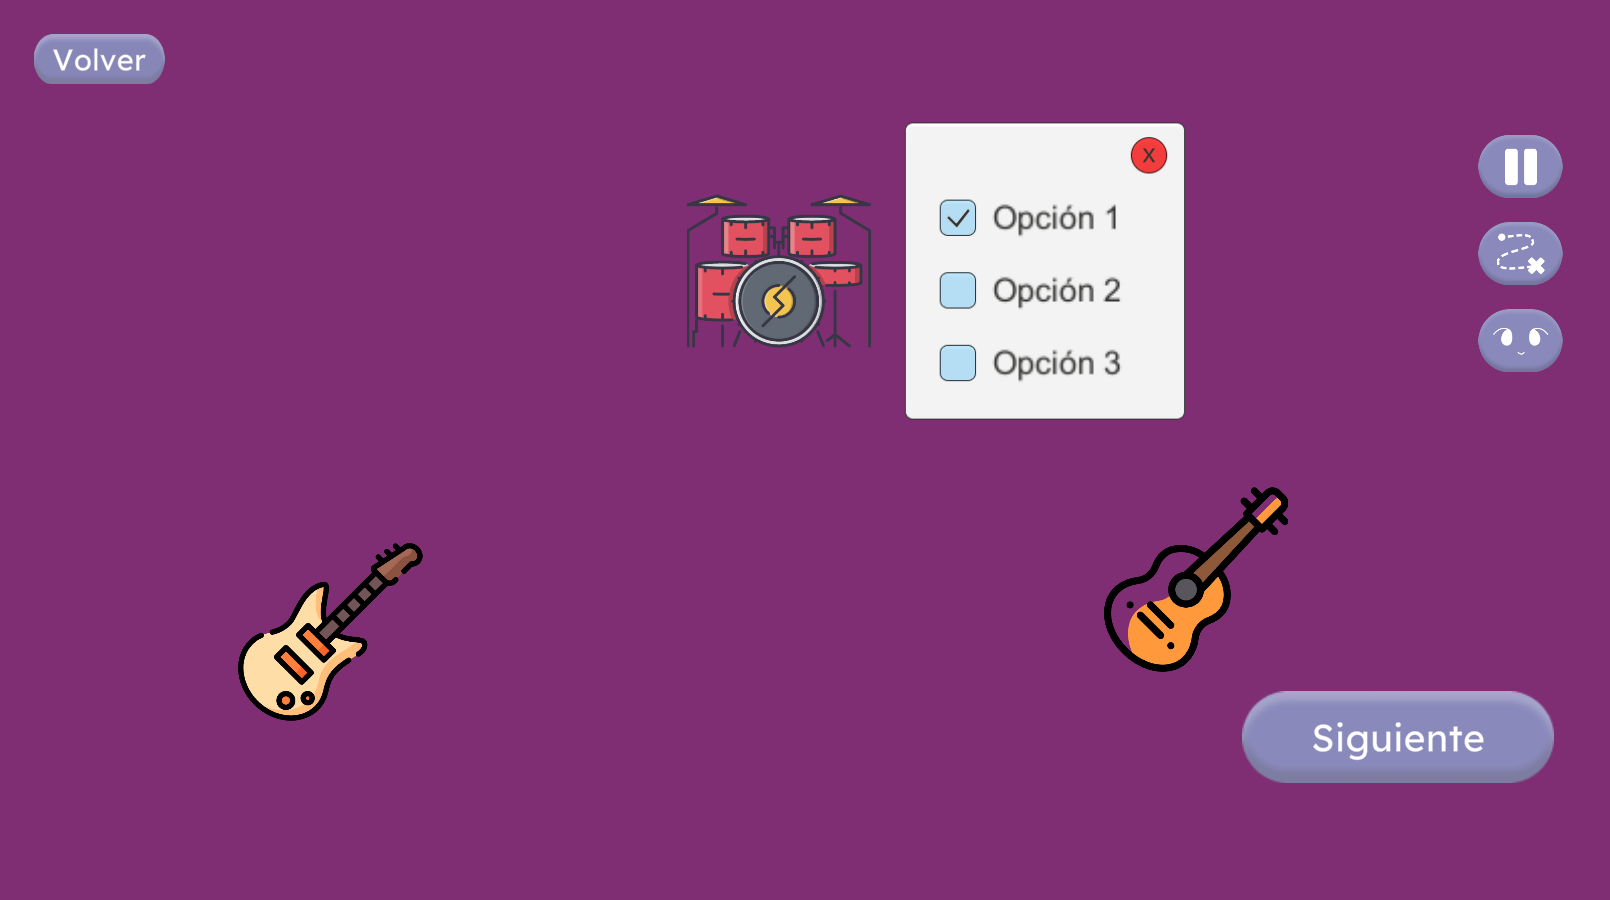
\includegraphics[width=0.4\textwidth]{./Figuras/Desarrollo/PaisajeSonoroGame.png}\label{fig:SonoricEnvironmentGame}}
	\caption{Pantallas del menú y del juego en la aplicación de paisaje sonoro.}
	\label{fig:SonoricEnvironment}
	\vspace{-30pt}
\end{figure}

\begin{center}
	\textbf{Fuente:} Realizado por Ángela García, miembro ARTEMIS.
\end{center}

\begin{figure}[h!]
	\centering
	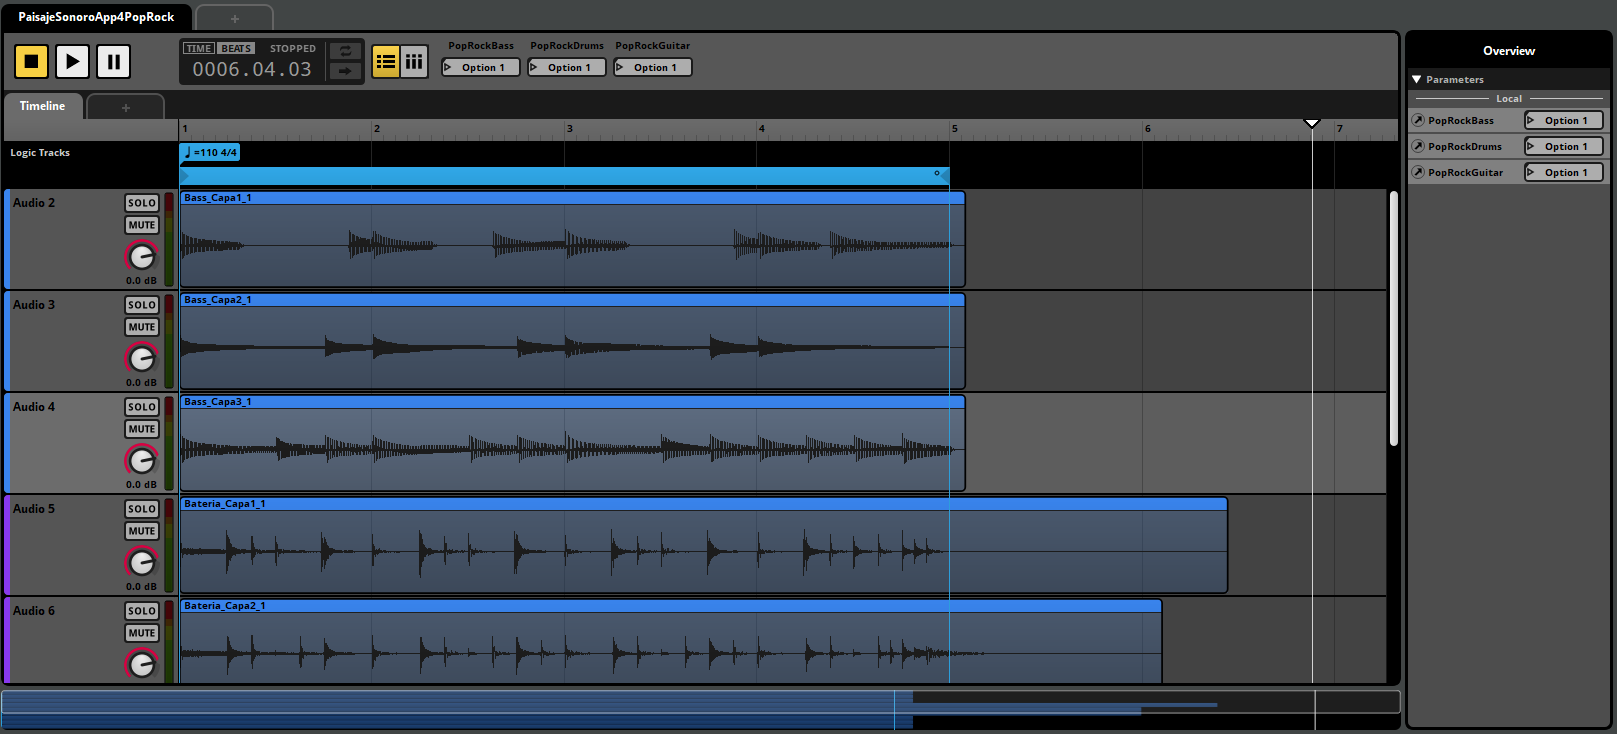
\includegraphics[width=0.8\linewidth]{Figuras/Desarrollo/PaisajeSonoroFMOD.png}
	\caption[Interfaz de FMOD aplicación paisaje sonoro.]{Interfaz de FMOD con los contenidos del género pop-rock de la aplicación de paisaje sonoro.}
	\label{fig:SonoricEnvironmentFMOD}
	\vspace{-40pt}
\end{figure}

\begin{center}
	\textbf{Fuente:} Realizado por Leticia Goás, compositora ARTEMIS.
\end{center}

A nivel musical, la aplicación utiliza FMOD para sincronizar rítmicamente las diversas pistas de audio y los parámetros para alternar entre ellas. Se puede observar en la \autoref{fig:SonoricEnvironmentFMOD}, cómo está configurado el middleware de audio para garantizar el correcto funcionamiento de la aplicación. Cada evento de FMOD engloba un género específico. Aquí se agrupan todas las pistas de audio por instrumentos, que se reproducen según los parámetros indicados a través de scripting dentro de Unity.

\subsection{Aplicación 2: Melodía floral}

A diferencia de la aplicación anterior, esta tiene una complejidad musical mayor, requiriendo un entendimiento teórico previo para su uso. Sin embargo, los conceptos utilizados en la aplicación son bastante sencillos para que un niño sin experiencia musical pueda aprenderlos rápidamente, tras una breve explicación del terapeuta. Al mismo tiempo, son lo suficientemente profundos para que un niño con experiencia musical pueda desenvolverse cómodamente con sus conocimientos adquiridos previamente. La aplicación de melodía floral incluye un pentagrama interactivo que permite cambiar tanto la duración como la altura de las notas. Por ello, es necesario conocer la nomenclatura musical, aunque no necesariamente de las notas, pero sí de los tipos de duración que existen, como las redondas, blancas, negras, corcheas, o incluso, los silencios.

\begin{figure}[h!]
	\centering
	\subfigure{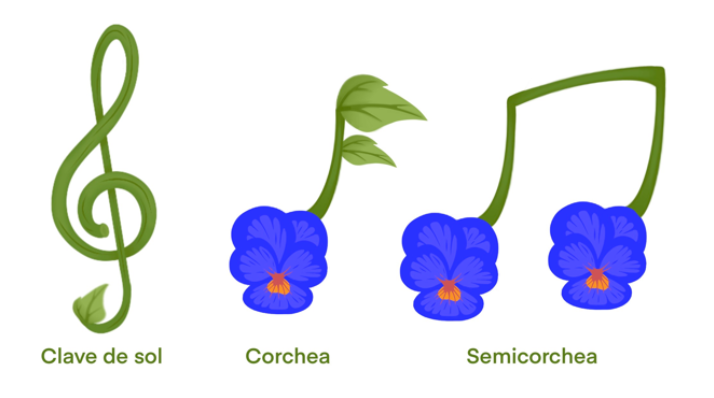
\includegraphics[width=0.45\textwidth]{./Figuras/Desarrollo/MelodiaFloralNotas1.png}\label{fig:FloralMelodyNotes1}}
	\subfigure{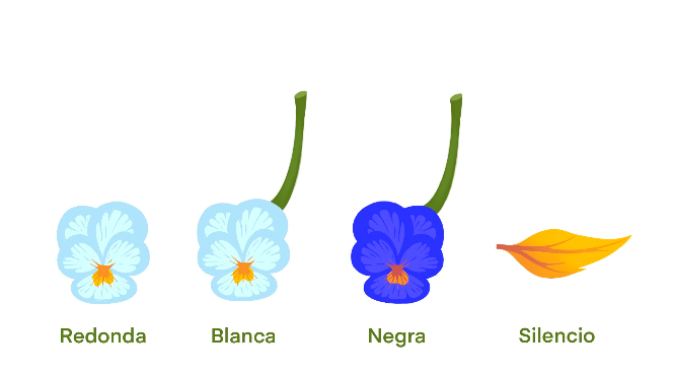
\includegraphics[width=0.45\textwidth]{./Figuras/Desarrollo/MelodiaFloralNotas2.png}\label{fig:FloralMelodyNotes2}}
	\caption{Representación visual de las figuras musicales en función de su duración.}
	\label{fig:FloralMelodyNotes}
	\vspace{-30pt}
\end{figure}

\begin{center}
	\textbf{Fuente:} Realizado por Isabel Xiaowei de San Sebastián, miembro ARTEMIS.
\end{center}

En cada iteración de la aplicación, se carga una melodía de una biblioteca, que el terapeuta puede seleccionar según las necesidades del paciente. Una vez seleccionada, aparece un pentagrama clásico con las notas dispuestas de acuerdo con la melodía. La estética de la aplicación conserva un aspecto natural, y cada nota se representa con un tipo de flor. La flor cambiará dependiendo de la duración de la nota, con las notas negras representadas por flores más oscuras y las notas blancas por flores literalmente blancas. Los silencios se representan con una hoja otoñal caída. Una gran referencia para la aplicación es el editor de melodías de \textit{Animal Crossing: New Horizons} (\cite{ACNH:2020}), que permite la creación musical a través de la colocación de notas y silencios, variando la altura de las mismas. 

Este enfoque visual ofrece varios beneficios terapéuticos. La representación visual de las notas como flores y hojas ayuda a los pacientes a conectarse emocionalmente con la música, haciendo que la experiencia sea más significativa. Además, la visualización de las notas y silencios facilita la comprensión de la teoría musical, incluso para aquellos sin conocimientos previos. La capacidad de crear y modificar melodías permite a los pacientes expresarse de manera creativa, lo cual puede ser especialmente útil para la liberación emocional y la exploración de sentimientos.

\begin{figure}[h!]
	\centering
	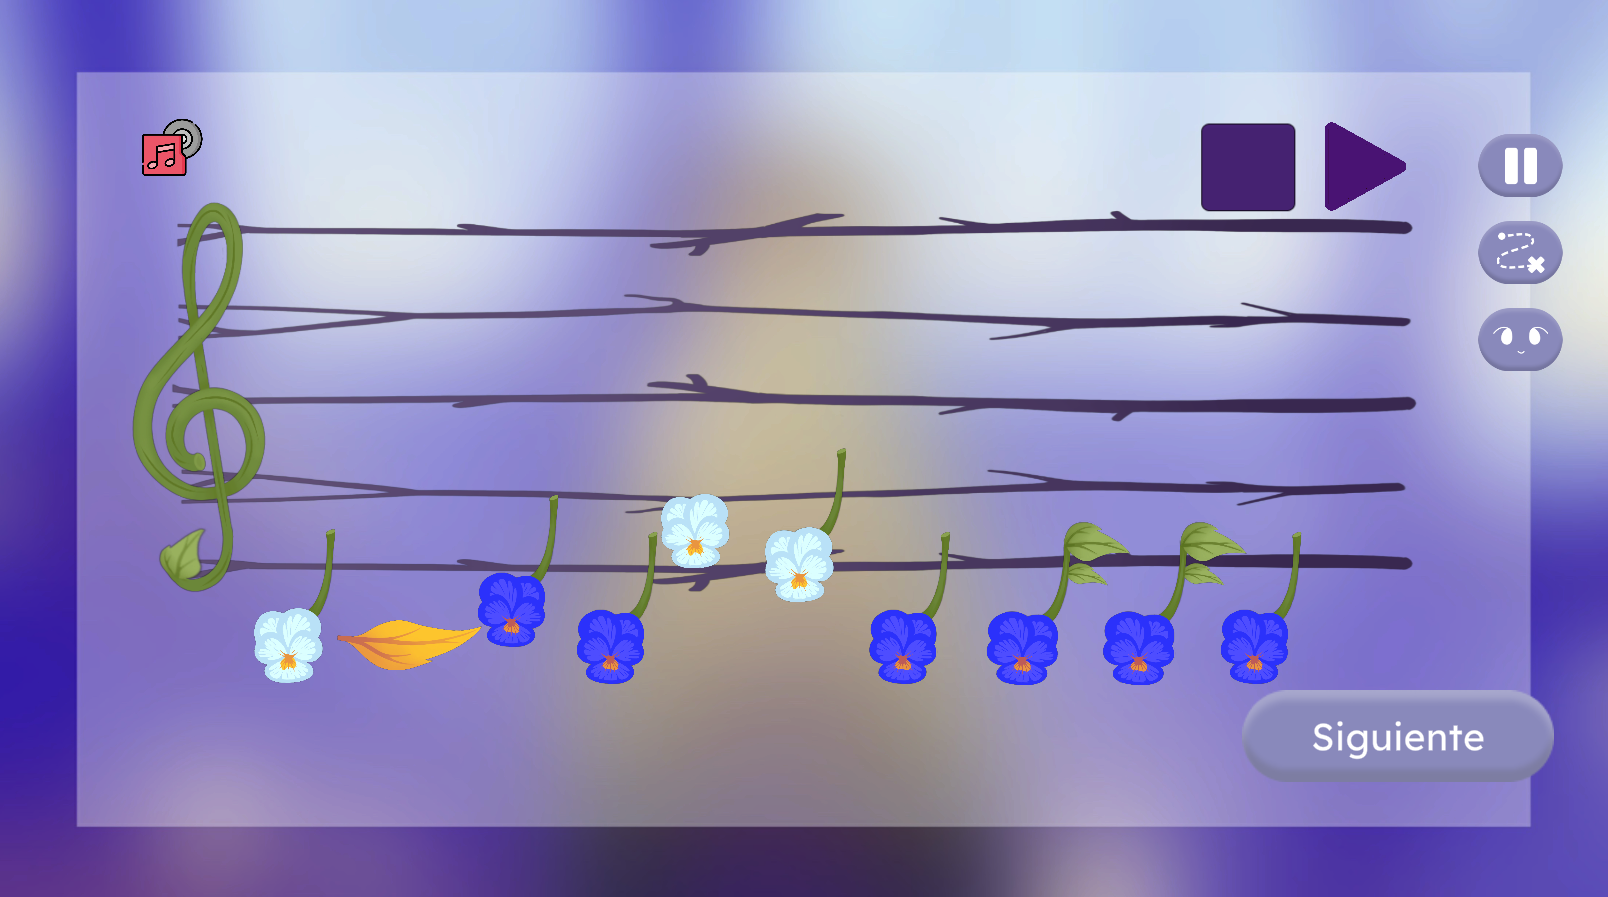
\includegraphics[width=0.8\linewidth]{Figuras/Desarrollo/MelodiaFloralGame.png}
	\caption[Interfaz de la aplicación melodía floral.]{Interfaz de la aplicación de melodía floral, mostrando un ejemplo de notas a distintas alturas y con diferentes figuras.}
	\label{fig:FloralMelodyGame}
	\vspace{-18pt}
\end{figure}

\begin{center}
	\textbf{Fuente:} Realizado por Elisa Alonso, miembro ARTEMIS.
\end{center}

En la \autoref{fig:FloralMelodyGame}, se muestra un ejemplo visual de una secuencia de notas con sus respectivas representaciones de duración. Cuando el usuario presiona el botón de inicio (triángulo equilátero horizontal), las notas se reproducirán una a una con las alturas correspondientes y la duración especificada. También es posible modificar las notas mientras la secuencia está en ejecución, lo que permite escuchar los cambios en tiempo real.

Ambas aplicaciones, con el objetivo de permitir que el paciente exprese sus sentimientos, utilizan una serie de elementos únicos que determinan la profundidad del diseño y los casos de uso. Estos elementos permiten al terapeuta adaptar la aplicación y darle al paciente la libertad de expresar cómo se siente. Además, estas aplicaciones no solo están diseñadas para terapias individuales, sino que también ofrecen posibilidades para terapias grupales, facilitando la colaboración y socialización a través de ciertas dinámicas de grupo. En el contexto grupal, estas aplicaciones permiten a los pacientes trabajar juntos en la creación de melodías y compartir sus experiencias emocionales, fortaleciendo así las relaciones interpersonales entre ellos y el terapeuta.

La composición interactiva busca crear un entorno seguro donde los pacientes pueden explorar libremente sus sentimientos, fomentando la autoexpresión. La musicoterapia se complementa significativamente con la composición interactiva digital, aprovechando la capacidad expresiva de la música en entornos digitales. Estos entornos permiten el uso de visuales emocionantes junto con sistemas modulares adaptables a diversas situaciones. En función de la creación musical del paciente y la información que este proporcione al terapeuta, se puede obtener información valiosa para adaptar con mayor facilidad las sesiones terapéuticas.

\section{Musicoterapia y diseño de videojuegos (serious games)}

El diseño de videojuegos y la musicoterapia pueden parecer campos distintos inicialmente, pero tienen varios puntos en común que los vuelven complementarios en un contexto terapéutico. Los videojuegos, diseñados para ser interactivos, mantienen la atención del usuario, siempre que el diseño sea adecuado. Esta interactividad puede ser aplicada en la musicoterapia para involucrar activamente a los pacientes en su terapia. La posibilidad de interactuar con el entorno digital hace la terapia más dinámica y atractiva para el paciente. Además, la gamificación de las terapias mejora la participación de los pacientes. Sin duda, el mayor desafío en la gamificación de terapias es lograr un equilibrio; el juego debe ser interesante pero sin llegar a frustrar al paciente. El objetivo de incorporar el diseño de videojuegos en las terapias de musicoterapia es motivar a los pacientes a participar activamente, con el fin de alcanzar sus objetivos terapéuticos.

Los videojuegos son conocidos por utilizar una combinación de elementos visuales y auditivos para crear experiencias inmersivas, combinadas con la interacción, que es lo que lo diferencia de otros formatos audiovisuales como el cine. En la musicoterapia, estos elementos pueden ser utilizados para fortalecer la conexión emocional del paciente con la música. La creación de estas experiencias interactivas sumergen al paciente en un entorno enriquecido que facilita la expresión emocional. Es importante enfatizar que la motivación que deben tener los pacientes debe ser intrínseca. No debe estar ligada a ninguna recompensa más allá del propio placer de disfrutar jugando. La herramienta tecnológica tiene como objetivo ser un complemento, y que el simple hecho de utilizarla pueda ayudar al paciente sin necesidad de recompensas adicionales. La verdadera recompensa radica en el tránsito emocional, de emociones con connotaciones negativas a emociones con connotaciones positivas. Estas aplicaciones funcionan como un doble usuario donde terapeuta y paciente interactúan para alcanzar los objetivos de la terapia. El videojuego actúa como un núcleo de cooperación entre ambas partes, guiados por el terapeuta, para obtener mejores resultados. Además, el diseño de terapias grupales fomenta la interacción social y el apoyo mutuo entre los pacientes. 

Esta línea de investigación, compuesta por dos aplicaciones, se basa en el diseño de videojuegos para crear experiencias interactivas que sean atractivas para el paciente y útiles para el terapeuta en su labor por dirigir la terapia. La primera aplicación, llamada Harmony Heaven, utiliza el concepto de la exploración como un puzle. La segunda aplicación, Ritmo Vegetal, presenta un puzle que consiste en resolver una situación aparentemente caótica, pero sin existir una solución incorrecta, ya que esta será subjetiva para el paciente. Nos centraremos en detallar la primera aplicación y dejaremos la segunda para más adelante en el documento. Esto se debe a que la segunda aplicación es la más relevante para este TFG, ya que constituye la base de todo el trabajo del autor en el proyecto ARTEMIS.

\subsection{Aplicación 1: Harmony Heaven}

Harmony Heaven se centra en la resolución de rompecabezas a través de la exploración. El paciente debe ayudar a un personaje a navegar por diferentes niveles que representan situaciones emocionales. Cada nivel se inicia con una emoción específica, en nuestro caso específico, la ansiedad. El objetivo es aprender a organizar y controlar los pensamientos y emociones para avanzar en el juego. Esto se logra a través de la resolución de un rompecabezas que, al ser ordenado, produce una melodía relajante. Los niveles, que cuentan con elementos del género de plataformas, tienen una jugabilidad en dos dimensiones. Harmony Heaven se inspira en juegos como \textit{Gris} (\citeauthor{GRIS:2018}, \citeyear{GRIS:2018}), \textit{Journey} (\citeauthor{JOURNEY:2012}, \citeyear{JOURNEY:2012}) y \textit{Flower} (\citeauthor{FLOWER:2009}, \citeyear{FLOWER:2009}), en términos de jugabilidad, estética y diseño sonoro.

\begin{figure}[h!]
	\centering
	\subfigure{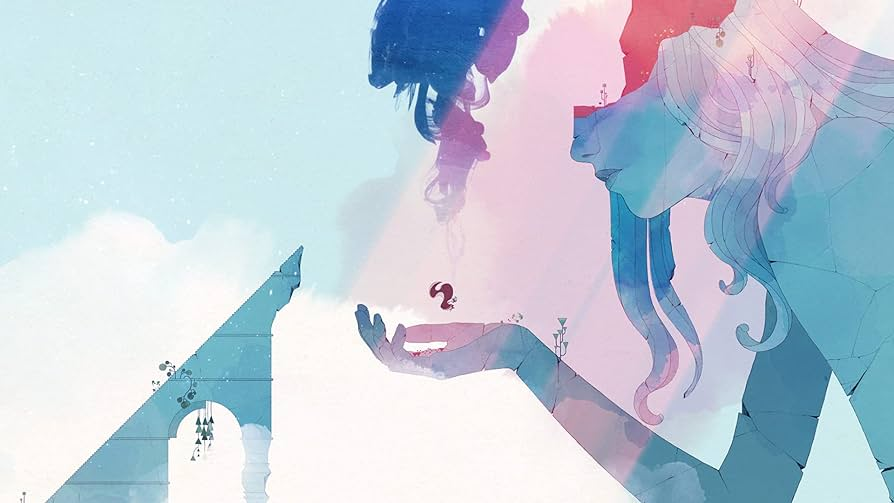
\includegraphics[width=0.29\textwidth]{./Figuras/Desarrollo/Gris.jpg}\label{fig:Gris}}
	\hfil
	\subfigure{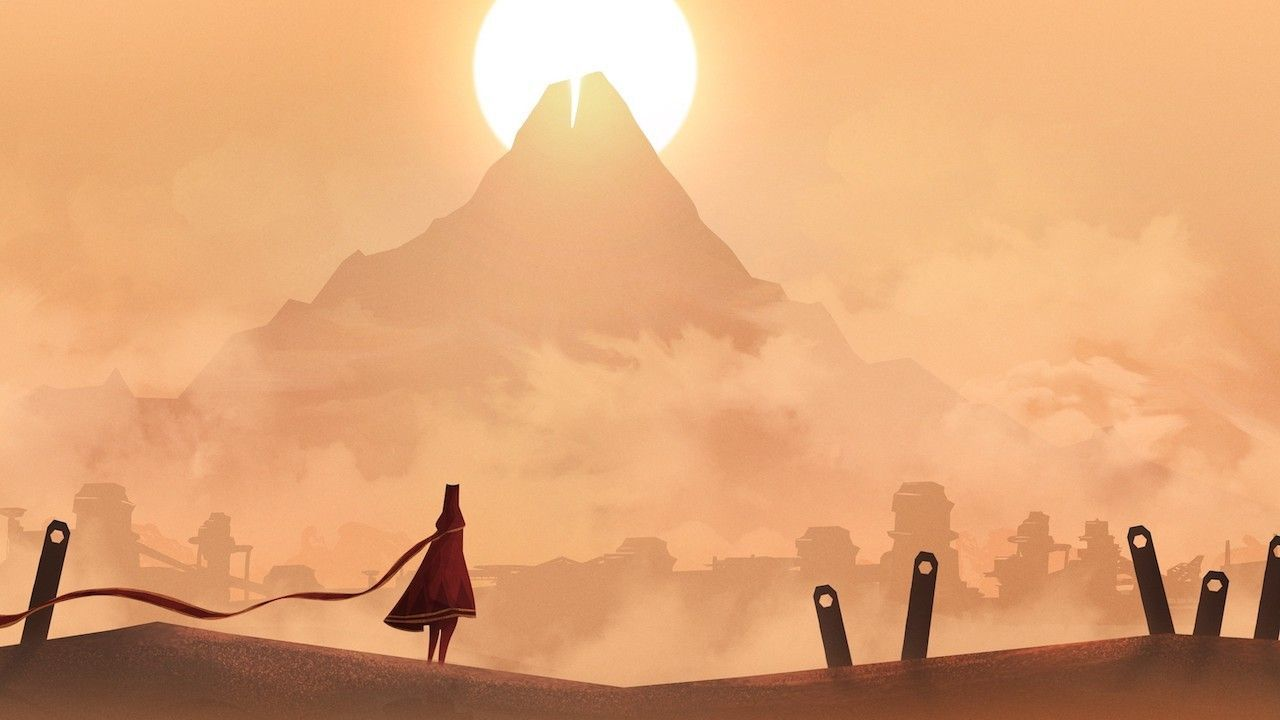
\includegraphics[width=0.29\textwidth]{./Figuras/Desarrollo/Journey.jpg}\label{fig:Journey}}
	\hfil
	\subfigure{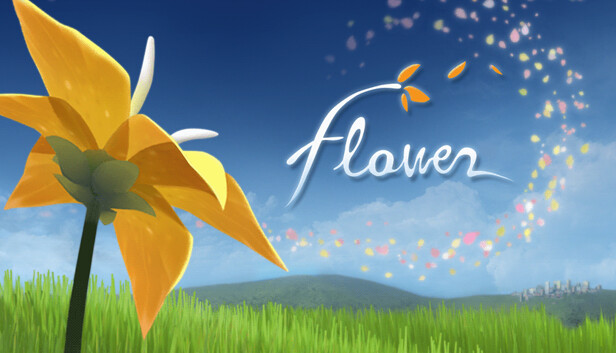
\includegraphics[width=0.29\textwidth]{./Figuras/Desarrollo/Flower.jpg}\label{fig:Flower}}
	\caption[Inspiraciones aplicación Harmony Heaven.]{Imágenes de referencia sobre las inspiraciones que se han tomado para Harmony Heaven.}
	\label{fig:HarmonyHeavenRefs}
	\vspace{-26pt}
\end{figure}

\begin{center}
	\textbf{Fuente:} Capturas recogidas de las respectivas páginas web. Se pueden encontrar en la referencia bibliográfica del videojuego.
\end{center}

\begin{figure}[h!]
	\centering
	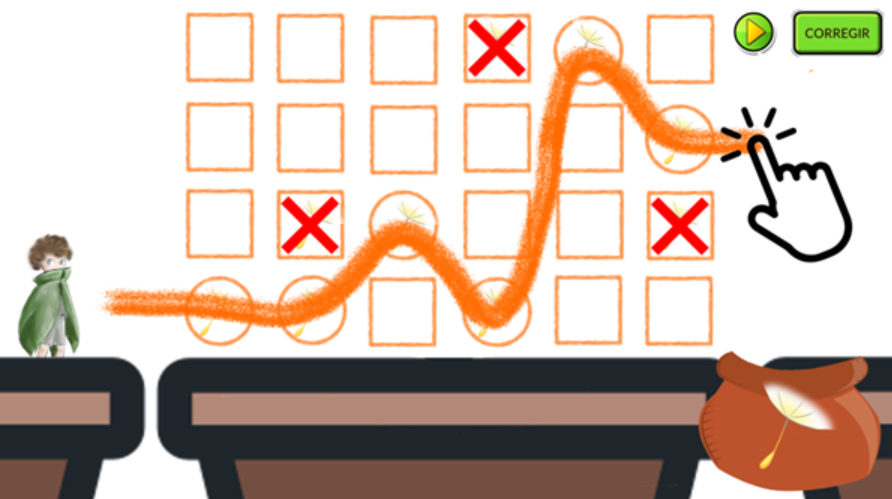
\includegraphics[width=0.7\linewidth]{Figuras/Desarrollo/HarmonyHeaven.png}
	\caption{Concepto de puzle de la aplicación Harmony Heaven.}
	\label{fig:HarmonyHeavenGame}
	\vspace{-30pt}
\end{figure}

\begin{center}
	\textbf{Fuente:} Realizado por Gonzalo Blanco, miembro ARTEMIS.
\end{center}

El puzle por exploración consta de dos partes. En la fase de exploración, el paciente debe buscar piezas ocultas, mientras que en la fase de resolución, estas piezas se utilizan para resolver un puzle musical. Las piezas deben colocarse a la altura correcta para que la melodía suene adecuadamente. Como se muestra en la \autoref{fig:HarmonyHeavenGame}, las piezas colocadas correctamente están rodeadas de un círculo, mientras que las 'X' marcan los lugares donde se ha cometido un error.

\section{UX/UI interacción y branding}

La línea de investigación de experiencia e interfaz de usuario se enfoca en la creación de la imagen de marca y en la integración interactiva de la aplicación, basándose en el estilo visual del proyecto. También se centra en realizar un trabajo detallado en la arquitectura de la información para garantizar que la interfaz de usuario sea intuitiva y fácil de navegar. Esto incluye la organización de menús, botones y otros elementos interactivos.

\begin{figure}[h!]
	\centering
	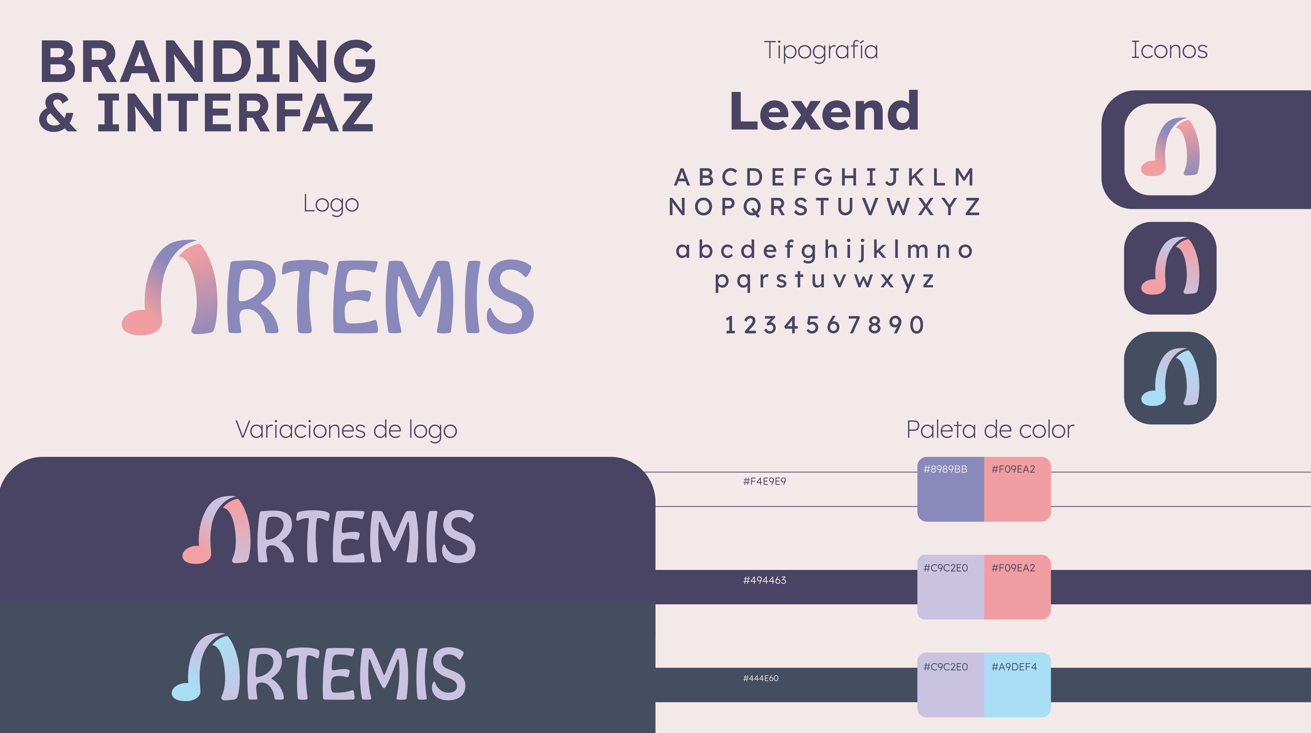
\includegraphics[width=\linewidth]{Figuras/Desarrollo/Branding.png}
	\caption{Imagen principal de marca del proyecto ARTEMIS.}
	\label{fig:Branding}
	\vspace{-26pt}
\end{figure}

\begin{center}
	\textbf{Fuente:} Realizado por Veja Zilakauskaite, miembro ARTEMIS.	
\end{center}

La \autoref{fig:Branding} contiene toda la información esencial sobre la imagen de marca del proyecto ARTEMIS. Esta incluye los logotipos e iconos, junto con la tipografía que se ha utilizado a lo largo del proyecto. El icono, que representa una nota musical con forma de 'A' derivada del nombre del proyecto, simboliza el objetivo del proyecto: la transición suave y progresiva entre emociones.

\section{Ritmo vegetal: Una experiencia rítmica para mejorar el bienestar emocional}

Esta sección es la más relevante del desarrollo de este TFG, ya que conforma todo el trabajo del autor y su tutor sobre el proyecto ARTEMIS. Discutiremos en detalle el proceso de desarrollo, enfocándonos en cada fase de la creación de la experiencia rítmica interactiva. El enfoque de este desarrollo, según la metodología descrita, se divide en varias fases comunes al desarrollo de videojuegos. Estas fases incluyen la preproducción y la producción. 

\subsection{Preproducción: Prerrequisitos}

El punto de partida de esta aplicación se ciñe a una serie de requisitos que fueron estipulados antes del comienzo del proyecto. El videojuego debía ser rítmico/musical para correlacionarse con la teoría y práctica de la musicoterapia, y ser compatible con este tipo de terapia. Además, tenía que ser modular para adaptarse a diferentes rangos de edades y emociones de estudio, si el proyecto escalaba en el futuro. También era importante que el jugador (paciente) no sólo interactuara, sino que también fuera creador, construyendo nuevos recursos a partir de los proporcionados por la experiencia. Por encima de todo, la aplicación debía alcanzar el objetivo principal del proyecto ARTEMIS: facilitar la transición de emociones con connotaciones negativas a emociones con connotaciones positivas. Se mencionan el término emociones con connotaciones dado que las emociones en sí mismas no son ni positivas ni negativas, aunque las connotaciones sí lo sean. En realidad, las emociones pueden ser potenciadoras o limitantes, y ambas son igual de importantes. Desde el principio, no se había decidido cuál sería la emoción a estudiar. Por lo tanto, se creó una tabla que comparaba las emociones limitantes con sus respectivas emociones potenciadoras, para facilitar la elección de esta.

\begin{table}[h!]
	\centering
	\resizebox{0.5\textwidth}{!}{
		\begin{tabular}{|c||c|}
			\hline
			\rowcolor[HTML]{FD6864} 
			\textbf{EMOCIÓN LIMITANTE} & \cellcolor[HTML]{9AFF99}{\color[HTML]{000000} \textbf{EMOCIÓN POTENCIADORA}} \\ \hline \hline
			Decepeción                 & Entusiasmo/Satisfacción                                                      \\ \hline
			Frustración/Indignación    & Motivación/Pasión/Ilusión                                                    \\ \hline
			Tristeza                   & Felicidad/Alegría                                                            \\ \hline
			Miedo                      & Bienestar                                                                    \\ \hline
			Soledad                    & Amor/Esperanza                                                               \\ \hline
			Asco                       & Afecto                                                                       \\ \hline
			Estrés/Ansiedad/Agobio     & Diversión/Humor                                                              \\ \hline
			Ira                        & Amor                                                                         \\ \hline
			Aburrimiento               & Diversión/Humor                                                              \\ \hline
			Preocupación               & Bienestar                                                                    \\ \hline
		\end{tabular}
	}
		\caption{Comparación de emociones limitantes contra sus respectivas potenciadoras.}
		\label{tab:Emotions}
		\vspace{-30pt}
\end{table}

\begin{center}
	\textbf{Fuente:} Realizado por el autor del TFG.	
\end{center}

Finalmente, decidimos que el objeto de estudio sería la ansiedad. Sin embargo, necesitábamos seleccionar un grupo social para esta primera iteración del proyecto. Al principio, consideramos que el grupo objetivo debería ser una población vulnerable. Los niños y ancianos parecían un buen punto de partida, pero notamos que, al ser un proyecto basado en tecnología interactiva digital, los niños tendrían una mayor facilidad de uso. Esto nos permitiría enfocarnos en el diseño de la experiencia terapéutica en lugar de adaptar la tecnología a un público específico, aunque no descartamos esta opción para el futuro. 

\subsection{Preproducción: Diseño conceptual}

Una vez definidos los prerrequisitos, el siguiente paso es diseñar conceptualmente la experiencia interactiva. El primer desafío que abordamos fue cómo hacer que el jugador (paciente) no solo sea un espectador pasivo de la aplicación, sino que se convierta en un creador activo. El objetivo es que el jugador se involucre más allá de simplemente jugar, sino también crear de manera que influya en el gameplay\footnote{El término gameplay se refiere a la parte jugable de un videojuego. Describe las reglas de funcionamiento y el diseño del videojuego específico al que se hace referencia.}. Un ejemplo ideal para ilustrar esta idea es \textit{Drawn To Life} (\cite{DTL:2007}), un videojuego en el que el jugador dibuja el personaje, como se puede observar en la \autoref{fig:DrawnToLife}, que luego utilizará en su aventura.

\begin{figure}[h!]
	\centering
	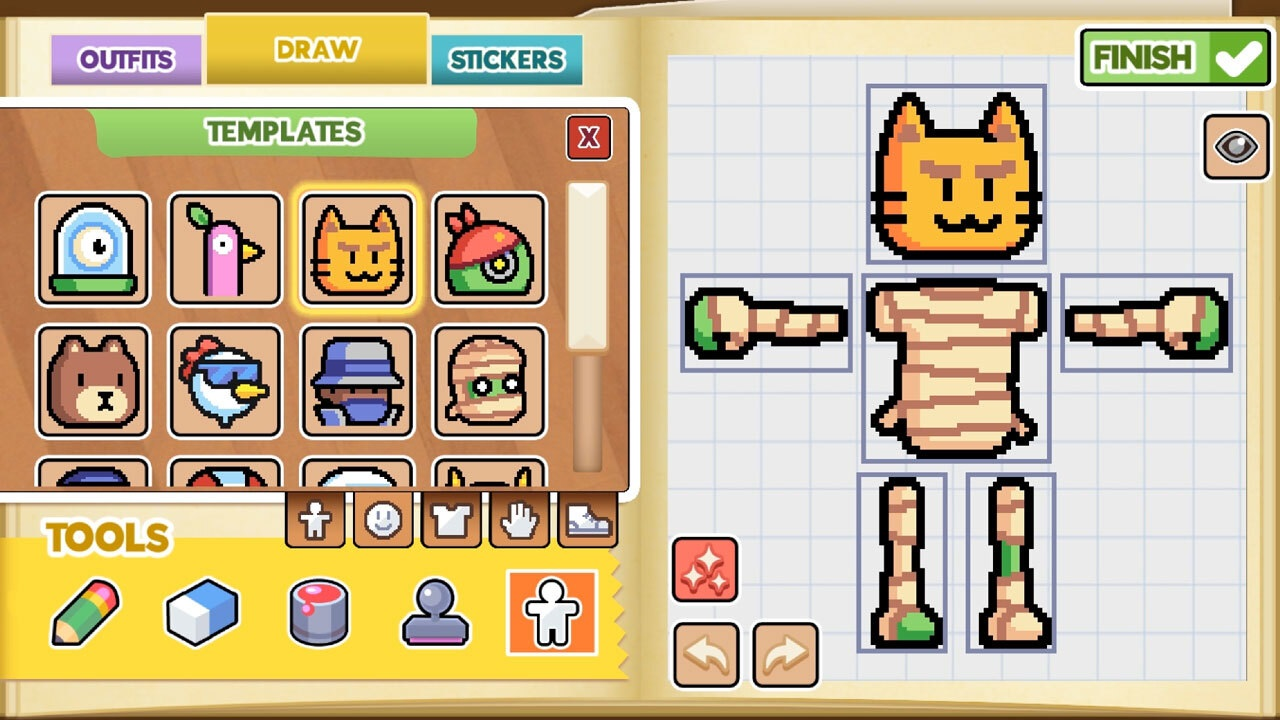
\includegraphics[width=0.7\linewidth]{Figuras/Desarrollo/DrawnToLife.jpg}
	\caption{Editor de personajes Drawn To Life.}
	\label{fig:DrawnToLife}
	\vspace{-30pt}
\end{figure}

\begin{center}
	\textbf{Fuente:} \citeauthor{DTL:2020} (\citeyear{DTL:2020}).
\end{center}

Para comenzar a conceptualizar un diseño de videojuego, primero recopilamos en una tabla una serie de referencias del género de los juegos de ritmo. La \autoref{tab:RhythmReferences} nos proporcionó una visión del estado actual del mercado de videojuegos en este género e inspiró algunas ideas para nuestro propio desarrollo.

\begin{table}[htbp]
	\centering
	\resizebox{\textwidth}{!}{
	\begin{tabular}{|l||l||c|}
		\hline
		\rowcolor[rgb]{ .788,  .761,  .878} \multicolumn{1}{|c|}{\textbf{Nombre}} & \multicolumn{1}{c|}{\textbf{Jugabilidad}} & \multicolumn{1}{c|}{\textbf{Link}} \\
		\hline
		\hline
		\textit{Arcaea (\cite{ARCAEA:2017})} & Similar a Piano Tiles, se incrementa la profundidad al añadir distintas alturas. & \multicolumn{1}{l|}{\textcolor[rgb]{ .02,  .388,  .757}{https://www.youtube.com/watch?v=ZcF9JQ44\_sw}} \\
		\hline
		\textit{Just Shapes \& Beats (\cite{JS&B:2018})} & Se basa en esquivar obstáculos, no necesariamente al ritmo de la música, aunque proporciona feedback visual acorde a la música. & \multicolumn{1}{l|}{\textcolor[rgb]{ .02,  .388,  .757}{https://www.youtube.com/watch?v=2VpqK2E8NRY}} \\
		\hline
		\textit{Beat Saber (\cite{BEATSABER:2018})} & Videojuego VR en el que deben romper los bloques al ritmo de la música. & \multicolumn{1}{l|}{\textcolor[rgb]{ .02,  .388,  .757}{https://www.youtube.com/watch?v=pa4vrynwkwY}} \\
		\hline
		\textit{BPM: Bullets Per Minute (\cite{BPM:2020})} & First Person Shooter en el que las acciones se deben realizar al ritmo de la música. & \multicolumn{1}{l|}{\textcolor[rgb]{ .02,  .388,  .757}{https://www.youtube.com/watch?v=cq-E6s91KyM}} \\
		\hline
		\textit{Crypt of the NecroDancer (\cite{COTN:2020})} & Las acciones están limitadas por casillas y se debe ritmo de la música. & \multicolumn{1}{l|}{\textcolor[rgb]{ .02,  .388,  .757}{https://www.youtube.com/watch?v=u\_avgU1u6yM}} \\
		\hline
		\textit{Cytus (\cite{CYTUS:2020})} & Similar a Osu!. & \multicolumn{1}{l|}{\textcolor[rgb]{ .02,  .388,  .757}{https://www.youtube.com/watch?v=k\_dibEIH4DE}} \\
		\hline
		\textit{Disaster Band (\cite{DISASTERBAND:2022})} & Similar a Trombone Champ pero cooperativo. & \multicolumn{1}{l|}{\textcolor[rgb]{ .02,  .388,  .757}{https://www.youtube.com/watch?v=prU6dtBEpCI}} \\
		\hline
		\textit{Elite Beat Agents (\cite{EBA:2005})} & Similar a Osu!. & \multicolumn{1}{l|}{\textcolor[rgb]{ .02,  .388,  .757}{https://www.youtube.com/watch?v=FDfKdrdRbkA}} \\
		\hline
		\textit{Friday Night Funkin' (\cite{FNF:2022})} & Similar a Piano Tiles. Caen flechas al ritmo de las canciones, teniendo apoyo visual con el movimiento de los personajes. & \multicolumn{1}{l|}{\textcolor[rgb]{ .02,  .388,  .757}{https://www.youtube.com/watch?v=xErhpjV8qNI}} \\
		\hline
		\textit{FUSER (\cite{FUSER:2020})} & Simulador de DJ. & \multicolumn{1}{l|}{\textcolor[rgb]{ .02,  .388,  .757}{https://www.youtube.com/watch?v=Ego\_IsxQw1I}} \\
		\hline
		\textit{Geometry Dash (\cite{GEOMETRYDASH:2013})} & Plataformas 2D con scroll lateral. Se deben esquivar obstáculos, y, en función del nivel, al ritmo de la música. & \multicolumn{1}{l|}{\textcolor[rgb]{ .02,  .388,  .757}{https://www.youtube.com/watch?v=k90y6PIzIaE}} \\
		\hline
		\textit{Guitar Hero Live (\cite{GUITARHEROLIVE:2015})} & Simulador de guitarra. & \multicolumn{1}{l|}{\textcolor[rgb]{ .02,  .388,  .757}{https://www.youtube.com/watch?v=YJgagY6j6ro}} \\
		\hline
		\textit{Hi-Fi Rush (\cite{HIFIRUSH:2023})} & Videojuego de aventura en tercera persona. Las acciones se deben realizar al ritmo de la música. & \multicolumn{1}{l|}{\textcolor[rgb]{ .02,  .388,  .757}{https://www.youtube.com/watch?v=\_GErIWYIhVc}} \\
		\hline
		\textit{The Impossible Game (\cite{IMPOSSIBLEGAME:2009})} & Plataformas 2D con scroll lateral. Se deben esquivar obstáculos, y, en función del nivel, al ritmo de la música. & \multicolumn{1}{l|}{\textcolor[rgb]{ .02,  .388,  .757}{https://www.youtube.com/watch?v=iQPEbHQZm68}} \\
		\hline
		\textit{Lost in Harmony (\cite{LIH:2016})} & Se basa en esquivar obstáculos, no necesariamente al ritmo de la música, aunque proporciona feedback visual acorde a la música. & \multicolumn{1}{l|}{\textcolor[rgb]{ .02,  .388,  .757}{https://www.youtube.com/watch?v=ZpumeaGwJvQ}} \\
		\hline
		\textit{Metal: Hellsinger (\cite{METALHELLSINGER:2022})} & First Person Shooter en el que las acciones se deben realizar al ritmo de la música. & \multicolumn{1}{l|}{\textcolor[rgb]{ .02,  .388,  .757}{https://www.youtube.com/watch?v=vzrFrhetMhA}} \\
		\hline
		\textit{Osu! (\cite{OSU!:2007})} & Los círculos se van cerrando y la interacción debe coincidir con el punto correcto de la canción. & \multicolumn{1}{l|}{\textcolor[rgb]{ .02,  .388,  .757}{https://www.youtube.com/watch?v=oI6X1pDMNlg}} \\
		\hline
		\textit{PaRappa The Rapper (\cite{PTR:2022})} & Juego de rap músical. & \multicolumn{1}{l|}{\textcolor[rgb]{ .02,  .388,  .757}{https://www.youtube.com/watch?v=y3SI4Grases}} \\
		\hline
		\textit{Patapon (\cite{PATAPON:2007})} & Videojuego 2D con scroll lateral. Se deben utilizar diferentes ritmos para  realizar diferentes acciones. & \multicolumn{1}{l|}{\textcolor[rgb]{ .02,  .388,  .757}{https://www.youtube.com/watch?v=Gvd21YW966A}} \\
		\hline
		\textit{Piano Tiles (\cite{PIANOTILES:2014})} & Videojuego con interacción táctil. Se debe presionar la tecla del piano en el momento indicado. & \multicolumn{1}{l|}{\textcolor[rgb]{ .02,  .388,  .757}{https://www.youtube.com/watch?v=kVIWzN0DmTc}} \\
		\hline
		\textit{Pistol Whip (\cite{PISTOLWHIP:2019})} & Videojuego VR en el que las acciones se deben realizar al ritmo de la música. & \multicolumn{1}{l|}{\textcolor[rgb]{ .02,  .388,  .757}{https://www.youtube.com/watch?v=mA75FYv6Nzg}} \\
		\hline
		\textit{Rhythm Heaven Fever (\cite{RHF:2011})} & Diferentes minijuegos rítmicos. & \multicolumn{1}{l|}{\textcolor[rgb]{ .02,  .388,  .757}{https://www.youtube.com/watch?v=2feG25a3VfQ}} \\
		\hline
		\textit{Sayonara Wild Hearts (\cite{SWH:2019})} & Movimiento híbrido 3D/2D en niveles musicales. & \multicolumn{1}{l|}{\textcolor[rgb]{ .02,  .388,  .757}{https://www.youtube.com/watch?v=F-RyxYcxSQ4}} \\
		\hline
		\textit{SingStar (\cite{SINGSTAR:2004})} & Simulador de canto. & \multicolumn{1}{l|}{\textcolor[rgb]{ .02,  .388,  .757}{https://www.youtube.com/watch?v=dNIOuio4-uU}} \\
		\hline
		\textit{Soundfall (\cite{SOUNDFALL:2022})} & Videojuego Hack\&Slash en el que las acciones se deben realizar al ritmo de la música. & \textcolor[rgb]{ .02,  .388,  .757}{https://www.youtube.com/watch?v=UhqempUAW2A} \\
		\hline
		\textit{Taiko no Tatsujin: Drum Session (\cite{TNTDS:2017})} & Videojuego de tambor rítmico. & \textcolor[rgb]{ .02,  .388,  .757}{https://www.youtube.com/watch?v=f7Yimxud4UI} \\
		\hline
		\textit{Theatrhythm Final Bar Line (\cite{TFBL:2023})} & Basado en el universo Final Fantasy, cuenta con diferentes minijuegos musicales. & \textcolor[rgb]{ .02,  .388,  .757}{https://www.youtube.com/watch?v=3EktIGradBI} \\
		\hline
		\textit{TLOZ: Cadence of Hyrule (\cite{TLOZCOH:2019})} & Las acciones están limitadas por casillas y se debe ritmo de la música. & \textcolor[rgb]{ .02,  .388,  .757}{https://www.youtube.com/watch?v=T2vSGCXkYac} \\
		\hline
		\textit{Trombone Champ (\cite{TROMBONECHAMP:2022})} & Se debe seguir la melodía de la música, con indicaciones lineales y progresivas, simulando un trombón. & \textcolor[rgb]{ .02,  .388,  .757}{https://www.youtube.com/watch?v=l-w5phrKu7Q} \\
		\hline
		\textit{VOEZ (\cite{VOEZ:2016})} & Piano Tiles avanzado donde se intercambian las líneas de notas. & \textcolor[rgb]{ .02,  .388,  .757}{https://www.youtube.com/watch?v=cInSMLRcvKo} \\
		\hline
	\end{tabular}
}
	\caption{Referencias de jugabilidad para el género de videojuegos musicales y de ritmo.}
	\label{tab:RhythmReferences}
	\vspace{-15pt}
\end{table}

\begin{center}
	\textbf{Fuente:} Realizado por el autor del TFG.
\end{center}

Después de analizar la situación actual de los videojuegos musicales, se propusieron dos conceptos de juego basados en los prerrequisitos, además de considerando las referencias anteriores. Ambas propuestas se centraban en la figura del paciente como creador, y no como únicamente jugador. El ciclo de juego en ambas propuestas debe ser corto, ya que se centra en terapias que suelen durar entre 30 y 60 minutos, compartiendo tiempo con otras actividades que el terapeuta considere adecuadas.

\begin{itemize}
	\item \textbf{Propuesta Beat 'Em Up:} esta propuesta se inspira en el clásico género Beat 'Em Up, donde el jugador avanza a través de un nivel lineal (comúnmente en dos dimensiones) derrotando enemigos en combate cuerpo a cuerpo. El bucle de juego se divide en dos fases:
	\begin{enumerate}
		\item \textbf{Fase de creación:} Al igual que un pedal de bucle para guitarras, que reproduce en bucle distintas iteraciones de lo que se toca en el instrumento, el jugador crea los comportamientos de los NPCs a través de varias iteraciones de jugabilidad. Estas iteraciones aumentan en duración hasta llegar a la versión final del personaje. El comportamiento de los NPCs se asemejaría a las sucesivas generaciones de una red neuronal, donde cada generación mejora a la anterior y optimiza su rendimiento en la tarea encomendada. La única diferencia radica en que, en las redes neuronales, el ajuste se realiza de manera aleatoria, basándose en una serie de parámetros establecidos por el usuario. Sin embargo, en nuestra propuesta, el control lo ejerce completamente el jugador. Cuando el jugador esté satisfecho con su creación, avanza a la siguiente fase con la versión del personaje que ha creado.
		
		\item \textbf{Fase de juego:} En esta fase, la jugabilidad se asemeja más a un Beat 'Em Up convencional, con la particularidad de que las acciones del jugador deben seguir el ritmo de la música. Patapon (\cite{PATAPON:2007}) es la principal referencia para entender esta jugabilidad rítmica.
	\end{enumerate}
	
	\begin{figure}[h!]
		\centering
		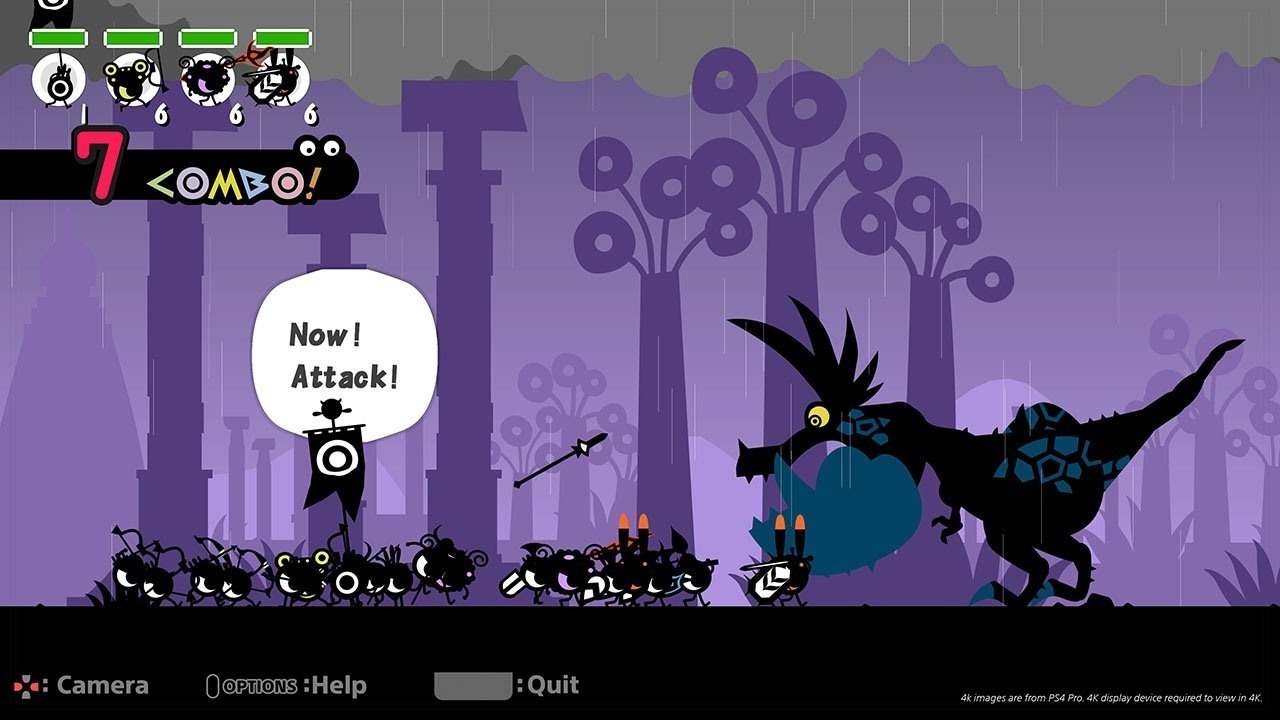
\includegraphics[width=0.6\linewidth]{Figuras/Desarrollo/Patapon.jpg}
		\caption{Referencia de jugabilidad de la fase de juego.}
		\label{fig:Patapon}
		\vspace{-30pt}
	\end{figure}
	
	\begin{center}
		\textbf{Fuente:} \citeauthor{PATAPON:2007} (\citeyear{PATAPON:2007}).
	\end{center}
	
	\item \textbf{Propuesta Lemmings:} esta propuesta se inspira en el clásico \textit{Lemmings} (\cite{LEMMINGS:1991}), en el cual el jugador debe ayudar a los pequeños personajes a alcanzar su meta, construyendo un camino seguro que les permita llegar a su destino. En nuestra propuesta específica, se propone la creación de un camino para que los personajes alcancen el punto final. Esto refuerza el prerrequisito del jugador como creador, pero además, la interacción de estos personajes con las plataformas producirá sonidos rítmicos o musicales, generando así música. Así, la creación no solo es una mecánica clave en la jugabilidad, sino que también se adapta para sesiones de musicoterapia, donde el paciente crea música mediante patrones rítmicos.
\end{itemize}

\begin{figure}[h!]
	\centering
	\subfigure{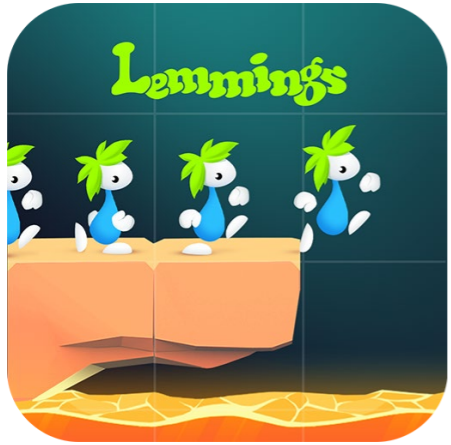
\includegraphics[width=0.29\textwidth]{./Figuras/Desarrollo/LemmingsLogo.png}\label{fig:LemmingsLogo}}
	\hfil
	\subfigure{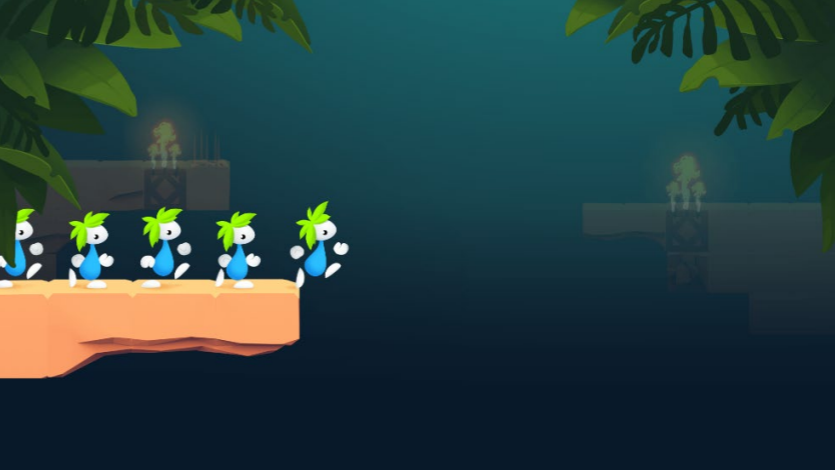
\includegraphics[width=0.5\textwidth]{./Figuras/Desarrollo/LemmingsGame.png}\label{fig:LemmingsGame}}
	\caption{Referencia de jugabilidad de la propuesta Lemmings.}
	\label{fig:Lemmings}
	\vspace{-30pt}
\end{figure}

\begin{center}
	\textbf{Fuente:} \citeauthor{LEMMINGS:2024} (\citeyear{LEMMINGS:2024}).
\end{center}

Al revisar ambas propuestas, se decidió que la de los Lemmings sería la elegida debido a su mejor adaptación al proyecto y a los intereses asociados, así como la cantidad de recursos necesarios para su realización. Este se convirtió en el punto de partida para las posteriores iteraciones hasta llegar al resultado final. La primera propuesta se desviaba más de los objetivos terapéuticos y requería más recursos para llevarse a cabo.

\subsection{Preproducción: Primeras iteraciones}

Basándonos en la propuesta seleccionada, realizamos una primera iteración considerando el contexto definido. El primer obstáculo que encontramos fue cómo adaptar las mecánicas del juego para que el ritmo fuera el elemento central. Decidimos que el espacio de juego sería una cuadrícula, debido a su semejanza con un pentagrama con sus respectivas líneas divisorias que separan los distintos compases (como se puede observar en la \autoref{fig:Pentagram}). En la sección \ref{code:grid}, se presenta el sistema de cuadrícula programado en C\#, el lenguaje que utiliza Unity. Asimismo, en la sección \ref{code:gridUtils}, se muestra una herramienta estática que facilita la creación de cada objeto que compone la cuadrícula. La combinación de ambos sistemas permite la creación de cuadrículas de diferentes tamaños. Este elemento de diseño refuerza la adaptabilidad para que el terapeuta pueda gestionar la dificultad de los niveles. Esto es importante en este tipo de terapias, como se observó en la investigación de la literatura.

\begin{figure}[h!]
	\centering
	
\includegraphics[width=0.8\linewidth]{Figuras/Desarrollo/Petagrama.png}
	\caption{Visualización del pentagrama con los distintos elementos que lo componen.}
	\label{fig:Pentagram}
	\vspace{-30pt}
\end{figure}

\begin{center}
	\textbf{Fuente:} \citeauthor{AUTODIDACTA:2020} (\citeyear{AUTODIDACTA:2020}).
\end{center}

En esta cuadrícula se colocan diferentes plataformas que producen sonidos variados dependiendo de la línea en la que se encuentren. El objetivo es simular la estructura de una partitura multi-instrumental, donde cada intérprete lee su línea específica para que, en conjunto, pueda sonar una pieza musical. Esta iteración concreta es la que más se asemeja al videojuego de referencia \textit{Lemmings} (\cite{LEMMINGS:1991}). El objetivo es ayudar a los personajes a cruzar el vacío, creando ritmos con las plataformas situadas en el entorno de juego. Para evitar la frustración del paciente, una plataforma colocada siempre se puede reubicar hasta que el paciente esté satisfecho con su creación.

\begin{figure}[h!]
	\centering
	\subfigure{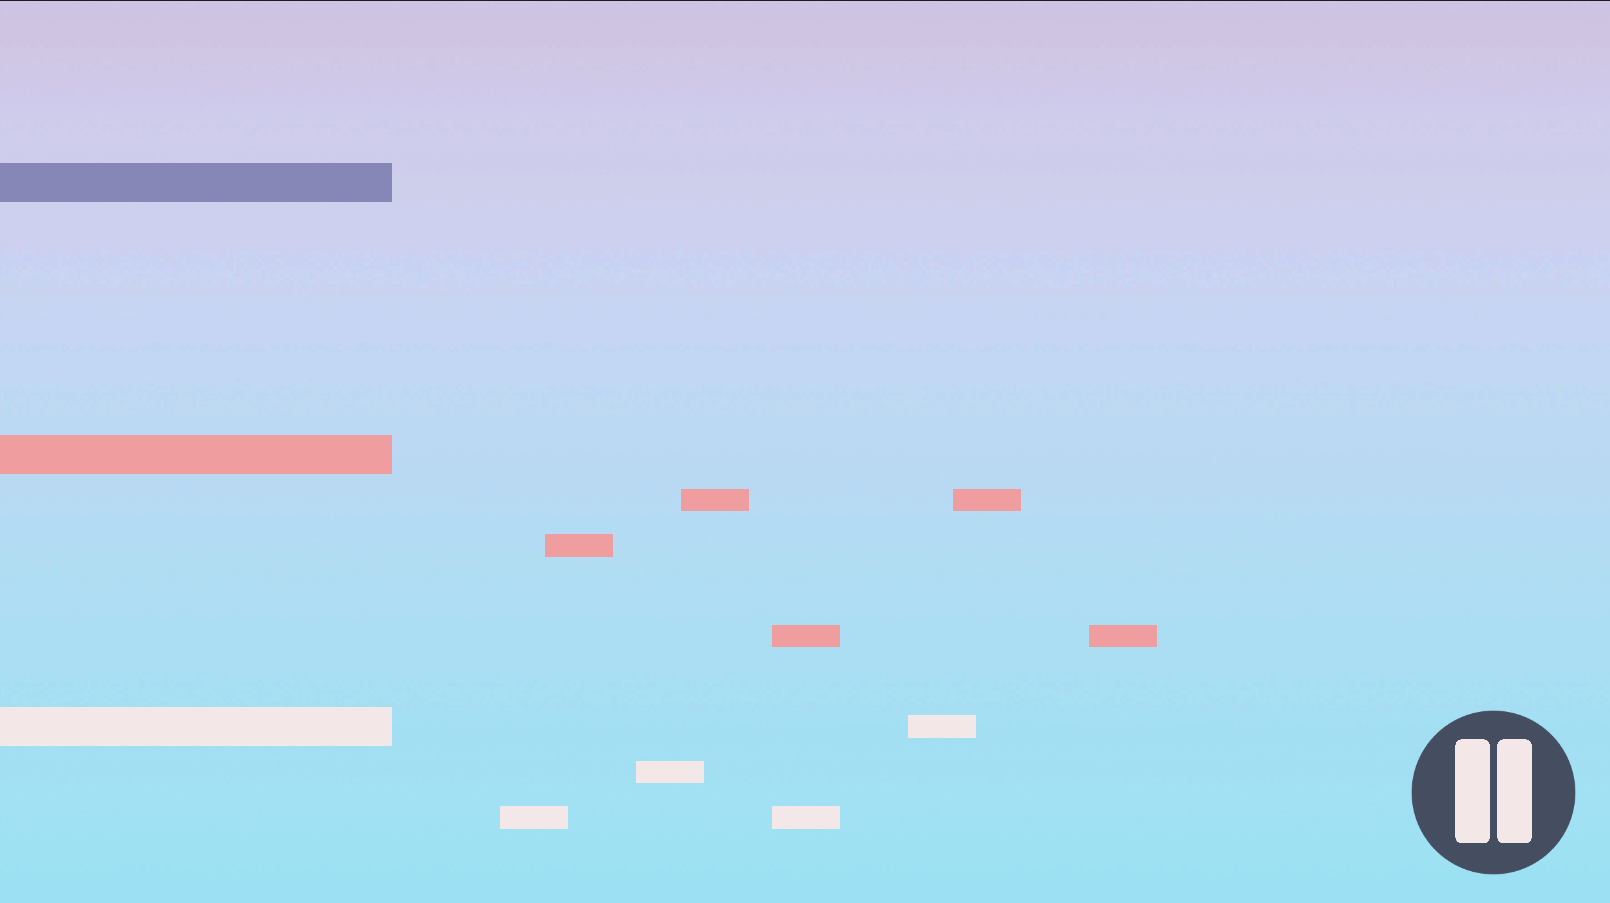
\includegraphics[width=0.45\textwidth]{./Figuras/Desarrollo/GridGame.png}\label{fig:GridGame}}
	\hfil
	\subfigure{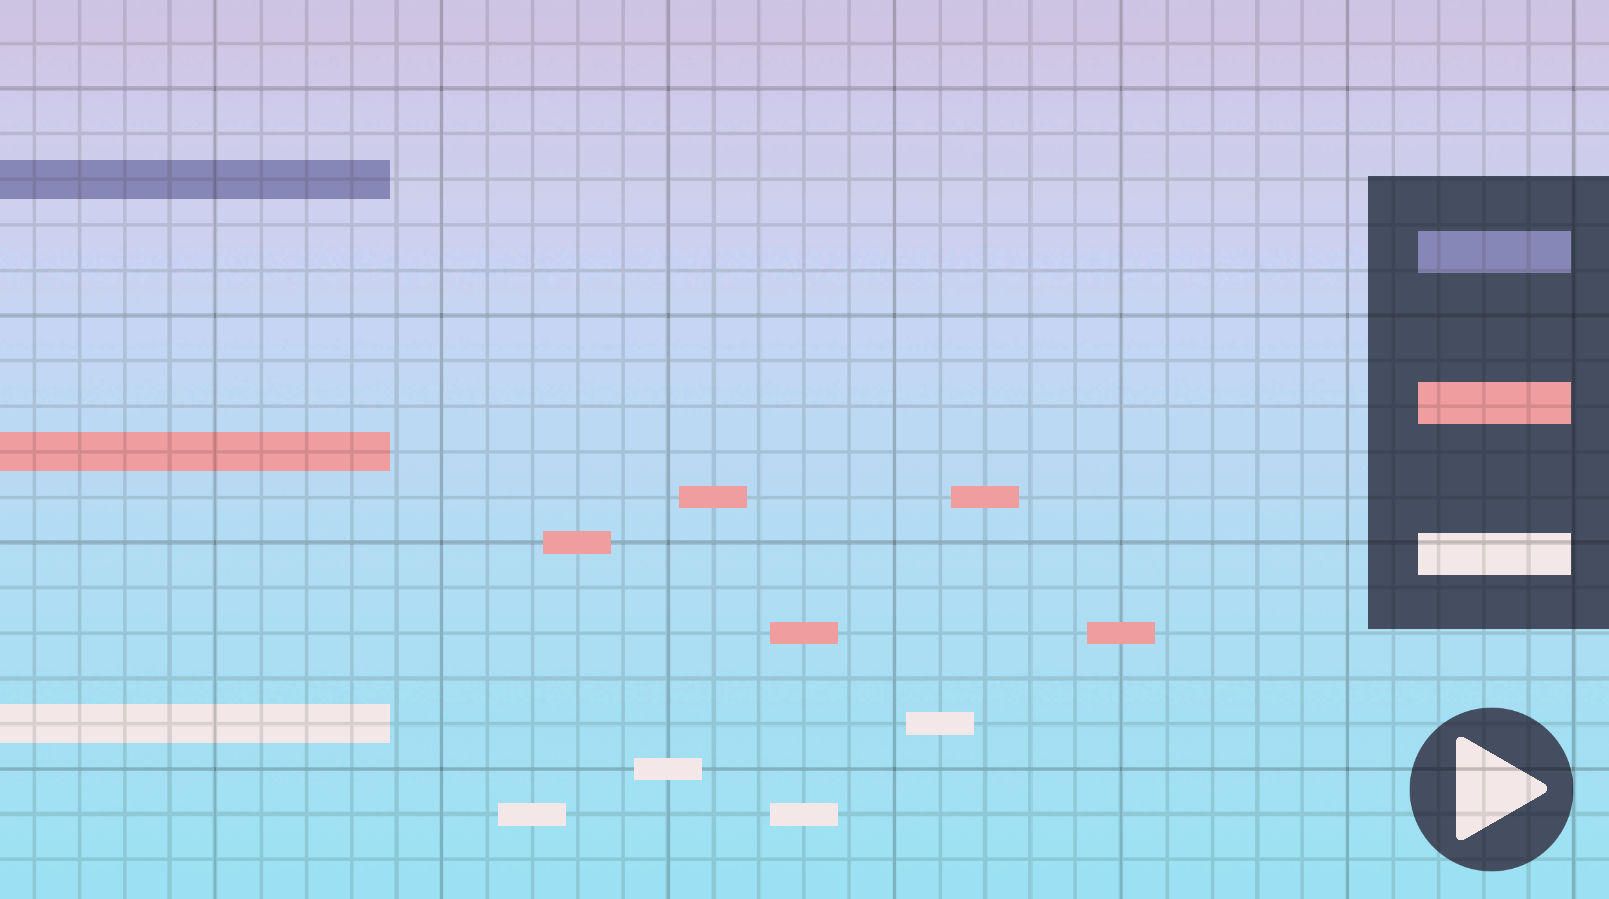
\includegraphics[width=0.45\textwidth]{./Figuras/Desarrollo/GridPause.png}\label{fig:GridPause}}
	\caption{Versión final de la primera iteración de la aplicación.}
	\label{fig:Grid}
	\vspace{-18pt}
\end{figure}

\begin{center}
	\textbf{Fuente:} Realizado por el autor del TFG.
\end{center}

En la \autoref{fig:Grid}, se presenta el entorno de juego. La jugabilidad se divide en dos fases: la fase de juego (\autoref{fig:GridGame}) y la fase de creación (\autoref{fig:GridPause}). Durante la fase de creación, el tiempo de juego se pausa y se permite al paciente colocar las plataformas a su gusto. Una vez que se reanuda el juego, el tiempo vuelve a fluir con normalidad y los personajes reaccionan a las colisiones con las nuevas plataformas, generando nuevos sonidos. Los recursos, es decir, las plataformas, son ilimitados. El paciente tiene a su disposición la cantidad de plataformas que necesite para crear música. La primera iteración presentó varios problemas. En términos de diseño, el paciente tendría demasiada libertad, lo que podría resultar en una sensación de abrumación similar a la que un escritor experimenta frente a una hoja en blanco. Muchas opciones posibles, pero poca claridad en la concreción de ideas. Además, la simultaneidad de instrumentos no produce una melodía clara, lo cual contradice nuestro objetivo de fomentar la relajación. Como resultado de estos problemas, surgió una segunda iteración centrada en simplificar las mecánicas y la melodía, permitiendo al paciente crear música mientras resuelve un rompecabezas con solución subjetiva.

En esta segunda iteración, las plataformas estarían ya posicionadas en el entorno de juego, eliminando la necesidad de la cuadrícula. Estas plataformas tendrían un movimiento restringido. Algunas solo podrían rotar, mientras que otras solo podrían desplazarse de manera horizontal, vertical, o en ambas direcciones. Los personajes caerían del cielo y al colisionar con las plataformas producirían diferentes sonidos, creando patrones rítmicos que se combinan con una melodía relajante. 

Esta última iteración evolucionó en la versión final de la aplicación. A continuación, se explicarán en detalle los aspectos de diseño y desarrollo, tanto mecánicos como musicales, de esta versión final. Todo lo redactado hasta este punto conduce a los siguientes apartados. Estos son el resultado de la combinación del trabajo del autor y su tutora, culminando en una versión final de la aplicación llamada \textit{Ritmo vegetal}.

\subsection{Producción: Decisiones de diseño}

La gracia del puzle está en resolverlo, motivación intrínseca.

\textbf{CONCLUSIONES}
INVESTIGACIONES FUTURAS